\documentclass[12pt, a4paper]{report}

\usepackage[utf8]{inputenc}
\usepackage[T1]{fontenc}
\IfFileExists{libertine.sty}{%
  \usepackage[mono=false]{libertine}%
  \IfFileExists{zi4.sty}{\usepackage[varqu]{zi4}}{}%
}{\usepackage{lmodern}%
}
\usepackage[protrusion=true, expansion=false]{microtype}
\usepackage[a4paper, width=155mm, top=25mm, bottom=25mm, headheight=15pt]{geometry}
\usepackage{setspace}
\onehalfspacing
\emergencystretch=3em
\hbadness=2000

\usepackage{amsmath,amssymb}
\usepackage{fontawesome5}
\newcommand{\tmarkDone}{\textbf{\faCheck}}
\newcommand{\tmarkNo}{\textbf{\faTimes}}
\newcommand{\tmarkPartial}{\faHourglassHalf}
\newcommand{\tmarkPlanned}{\textcolor{black!55}{\faCircle}}
\usepackage{graphicx}
% Figure sources: SVG in overleaf/ (symlink → Diagrams/); PDFs built by build-improved-diagrams.sh.
\newcommand*{\ThesisDiagDir}{overleaf/}
\graphicspath{{overleaf/}{./}}
\pdfimageresolution=300
\makeatletter
\newcommand*{\@thesis@doinclude}[2]{%
  \if\relax\detokenize{#1}\relax
    \includegraphics{#2}%
  \else
    \includegraphics[#1]{#2}%
  \fi
}
\newcommand*{\@thesismissingimg}[1]{%
  \fbox{\parbox{0.92\linewidth}{\scriptsize\centering\ttfamily Missing file: \detokenize{#1}.\\[2pt]Add it to the \texttt{overleaf/} folder and recompile.}}%
}
\newcommand{\ThesisIncludeGraphics}[2][]{%
  \IfFileExists{\ThesisDiagDir#2}{%
    \@thesis@doinclude{#1}{\ThesisDiagDir#2}}{%
  \IfFileExists{#2}{%
    \@thesis@doinclude{#1}{#2}}{%
    \@thesismissingimg{#2}%
  }}%
}
\makeatother
\newcommand{\TableScreenshotEnd}[2][]{%
  \refstepcounter{table}%
  \if\relax\detokenize{#1}\relax\else\label{#1}\fi%
  \phantomsection%
  \addcontentsline{lot}{table}{\protect\numberline{\thetable}#2}%
}
\usepackage[table]{xcolor}
\usepackage{tikz}
\usetikzlibrary{arrows.meta,positioning,fit,shapes.geometric,calc}
\usepackage{pgfplots}
\usepgfplotslibrary{statistics}
\pgfplotsset{compat=1.18, minor tick num=0}

\usepackage{booktabs}
\usepackage{array}
\usepackage{colortbl}
\usepackage{multirow}
\usepackage{float}
\usepackage{etoolbox}
\usepackage{caption}
\captionsetup{
    labelfont={bf,small},
    textfont={small},
    skip=6pt,
    format=hang
}
\makeatletter
% Compact, professional List of Figures / List of Tables (no tocloft dependency)
\renewcommand*\l@figure{\@dottedtocline{1}{0em}{3.2em}}
\renewcommand*\l@table{\@dottedtocline{1}{0em}{3.8em}}
\makeatother

\newlength{\ThesisTableImgReserve}
\newlength{\ThesisFigImgReserve}
\setlength{\ThesisTableImgReserve}{\dimexpr2\intextsep+0.75\baselineskip\relax}
\setlength{\ThesisFigImgReserve}{\dimexpr2\intextsep+\abovecaptionskip+\belowcaptionskip+4\baselineskip\relax}
\newcommand{\TableImageMaxFit}[1]{%
  \ThesisIncludeGraphics[
    width=0.7\linewidth,
    height=\dimexpr(\textheight-\ThesisTableImgReserve)*7/10\relax,
    keepaspectratio
  ]{#1}%
}
\newcommand{\FigureImageMaxFit}[1]{%
  \ThesisIncludeGraphics[width=\linewidth,height=\dimexpr\textheight-\ThesisFigImgReserve\relax,keepaspectratio]{#1}%
}
\newcommand{\OnePageDiagram}[2][]{%
  \if\relax\detokenize{#1}\relax
    \ThesisIncludeGraphics[width=\linewidth,height=\dimexpr\textheight-\ThesisFigImgReserve\relax,keepaspectratio]{#2}%
  \else
    \ThesisIncludeGraphics[#1,width=\linewidth,height=\dimexpr\textheight-\ThesisFigImgReserve\relax,keepaspectratio]{#2}%
  \fi
}
\newcommand{\HalfWidthDiagram}[1]{%
  \ThesisIncludeGraphics[width=0.5\linewidth, keepaspectratio]{#1}%
}
\newcommand{\WideDiagram}[2][]{%
  \if\relax\detokenize{#1}\relax
    \ThesisIncludeGraphics[width=\linewidth, height=0.78\textheight, keepaspectratio]{#2}%
  \else
    \ThesisIncludeGraphics[#1, width=\linewidth, height=0.78\textheight, keepaspectratio]{#2}%
  \fi
}
\newcommand{\TallDiagram}[2][]{%
  \if\relax\detokenize{#1}\relax
    \ThesisIncludeGraphics[width=\linewidth, height=0.96\textheight, keepaspectratio]{#2}%
  \else
    \ThesisIncludeGraphics[#1, width=\linewidth, height=0.96\textheight, keepaspectratio]{#2}%
  \fi
}
% Balanced layout slot (reference: Figure 4.3 ml-explainability) — wide banded diagrams.
\newcommand{\BalancedDiagram}[2][]{%
  \if\relax\detokenize{#1}\relax
    \ThesisIncludeGraphics[width=\linewidth, height=0.72\textheight, keepaspectratio]{#2}%
  \else
    \ThesisIncludeGraphics[#1, width=\linewidth, height=0.72\textheight, keepaspectratio]{#2}%
  \fi
}
% Activity diagrams — full-height slot for 3× label size.
\newcommand{\ActivityDiagram}[2][]{%
  \if\relax\detokenize{#1}\relax
    \ThesisIncludeGraphics[width=\linewidth, height=\textheight, keepaspectratio]{#2}%
  \else
    \ThesisIncludeGraphics[#1, width=\linewidth, height=\textheight, keepaspectratio]{#2}%
  \fi
}
% Half-size slot (50\% of BalancedDiagram width and height).
\newcommand{\CompactDiagram}[2][]{%
  \if\relax\detokenize{#1}\relax
    \ThesisIncludeGraphics[width=0.5\linewidth, height=0.36\textheight, keepaspectratio]{#2}%
  \else
    \ThesisIncludeGraphics[#1, width=0.5\linewidth, height=0.36\textheight, keepaspectratio]{#2}%
  \fi
}
\usepackage[skins]{tcolorbox}
% Empty slot for figures pending vector artwork (no PNG in thesis).
\newcommand{\FigurePlaceholder}[1][0.72\textheight]{%
  \begin{tcolorbox}[colback=white,colframe=gray!35,boxrule=0.4pt,arc=0pt,
    width=\linewidth,height=#1,halign=center,valign=center]
    \mbox{}
  \end{tcolorbox}
}

\usepackage{titlesec}
\usepackage{parskip}
\usepackage{fancyhdr}
\usepackage{enumitem}
\PassOptionsToPackage{hyphens,spaces,obeyspaces}{url}
\usepackage{hyperref}
\makeatletter
\g@addto@macro\UrlBreaks{\do\/\do\-\do\.\do\:\do\&\do\=\do\#}
\makeatother

\definecolor{PrimaryBlue}{HTML}{000000}
\definecolor{AccentBlue}{gray}{0.55}
\definecolor{LightBlue}{gray}{0.96}
\definecolor{MidBlue}{gray}{0.90}
\definecolor{DarkText}{HTML}{000000}
\definecolor{GrayText}{gray}{0.45}
\definecolor{RowShade}{gray}{0.965}
\definecolor{RowShadeAlt}{gray}{0.92}
\definecolor{TableHeadBg}{gray}{0.88}
\definecolor{TableRule}{gray}{0.55}
\definecolor{GreenAccent}{HTML}{000000}
\definecolor{AmberAccent}{HTML}{000000}
\definecolor{RedAccent}{HTML}{000000}
\definecolor{VioletAccent}{HTML}{000000}

\hypersetup{
    colorlinks=true,
    linkcolor=black,
    filecolor=black,
    urlcolor=black,
    citecolor=black,
    pdfborder={0 0 0},
}

\titleformat{\chapter}[display]
    {\normalfont\LARGE\bfseries}
    {\chaptertitlename\ \thechapter}{20pt}{\LARGE}
    [\vspace{4pt}{\color{black!40}\titlerule[0.6pt]}]

\titleformat{\section}
    {\large\bfseries}
    {\thesection}{0.8em}{}

\titleformat{\subsection}
    {\normalsize\bfseries}
    {\thesubsection}{0.6em}{}

\titleformat{\subsubsection}
    {\normalsize\bfseries\itshape}
    {\thesubsubsection}{0.6em}{}

\titlespacing*{\chapter}{0pt}{-20pt}{20pt}
\titlespacing*{\section}{0pt}{16pt plus 3pt minus 2pt}{8pt plus 2pt minus 1pt}
\titlespacing*{\subsection}{0pt}{12pt plus 2pt minus 1pt}{6pt plus 1pt minus 1pt}
\titlespacing*{\subsubsection}{0pt}{10pt plus 2pt minus 1pt}{4pt plus 1pt minus 1pt}

\newcommand{\tableheadcolor}{\rowcolor{TableHeadBg}}
\newcommand{\tableheadfont}{\bfseries}
\newcommand{\ThesisTableBodyFont}{\small}

% Consistent greyscale table polish (font size unchanged; spacing only).
\newcommand{\ThesisTablePrep}{%
  \ThesisTableBodyFont
  \renewcommand{\arraystretch}{1.22}%
  \setlength{\tabcolsep}{6pt}%
  \arrayrulecolor{TableRule}%
  \setlength{\aboverulesep}{0.55ex}%
  \setlength{\belowrulesep}{0.55ex}%
}
\AtBeginEnvironment{table}{\ThesisTablePrep}
\AtBeginEnvironment{tabular}{%
  \rowcolors{2}{}{RowShade}%
  \arrayrulecolor{TableRule}%
}

\newenvironment{moderntable}[1][H]{%
    \begin{table}[#1]\centering\ThesisTablePrep
}{%
    \end{table}%
}

\newtcolorbox{layerbox}[1]{
    colback=white,
    colframe=black!55,
    coltitle=black,
    fonttitle=\bfseries\small,
    title=#1,
    boxrule=0.6pt,
    arc=2pt,
    left=6pt,right=6pt,top=4pt,bottom=4pt,
}

\newtcolorbox{highlightbox}[1][]{
    colback=black!4,
    colframe=black!45,
    boxrule=0.5pt,
    arc=2pt,
    left=8pt,right=8pt,top=6pt,bottom=6pt,
    #1
}

\newtcolorbox{chapterinstruction}[2][]{%
  colback=black!4,colframe=black!55,title={#2},fonttitle=\bfseries\small,
  arc=2pt,left=8pt,right=8pt,top=6pt,bottom=6pt,#1}

\pagestyle{fancy}
\fancyhf{}
\renewcommand{\headrulewidth}{0.4pt}
\fancyhead[L]{\small\color{black!55}Crypto World Bank --- Heavily Compressed}
\fancyhead[R]{\small\color{black!55}BRAC University}
\fancyfoot[C]{\small\color{black!55}\thepage}

\begin{document}

\thispagestyle{empty}
\begin{center}
\vspace*{2cm}
{\LARGE\bfseries Decentralized Crypto World Bank}\\[0.5em]
{\large Heavily Compressed Pre-Thesis (v31)}\\[1.5em]
{\normalsize Md.\ Bokhtiar Rahman Juboraz \quad|\quad Md.\ Mahir Ahnaf Ahmed}\\[0.5em]
{\small BRAC University --- February 2026}
\end{center}
\newpage

\setcounter{page}{1}
\pagenumbering{roman}
\tableofcontents
\newpage
\listoffigures
\newpage
\pagenumbering{arabic}
\setcounter{page}{1}

\chapter{Introduction}
\label{sec:intro}

The \textit{Crypto World Bank} is a research-based project for exploring how blockchain technology can be shaped to fit into institutional financial systems with all the added benefits that come with a decentralized financing system. Based on our findings that had similar motivation to our study, existing DeFi protocols show isolated functionalities, such as Aave for lending, Uniswap for exchange, and MakerDAO for stablecoins. This project specifies a tier-based, hierarchically governed platform that includes a mixture of institutional financing with DeFi, accommodating deposit mobilization, credit allocation, interbank liquidity, installment repayment, FX facilitation, solidarity group lending, reserve enforcement, syndicated co-lending, and risk-based governance covering all four tiers that systematically mirrors real-world institutional financing. At the top, Tier~1 represents the World Bank reserve; the core banking hierarchy is specified in Solidity and being improved until final deployment. Another significant feature---the multi-entity contract suite---is fully specified in Chapter~3, which is scheduled for practical development in Phases~II--III.

The system is designed for three categories of participant: a programmable World Bank reserve as Tier~1, national and local development banks serving in Tiers~2--3, and retail clients in Tier~4. Retail clients get access to savings, group loans, and installment lending features. This hierarchical structure in this project was motivated by unbanked and MSME financing gaps~[9--10]. The project is not built with any motivation to deploy only in regions with access to advanced technologies; rather, proper distribution of access to finance and fairness is the leading cause of this attempt to find suitable ground to adapt DeFi among the general population. The whole project is open source and available in our \href{https://github.com/Yuvraajrahman/Cryto-World-Bank}{GitHub repository}. The added benefits of blockchain: it provides state visibility, tamper-evident audit trails, and programmable rule enforcement among institutions having competition, as demonstrated by the renowned World Bank FundsChain programme and JPMorgan Kinexys. From the study of institutions, open ledger infrastructure and institutional hierarchy are not mutually exclusive.

\begin{figure}[H]
\centering
\BalancedDiagram{Ch1_system-overview-four-tier-stack.pdf}
\caption[Crypto World Bank system overview]{Crypto World Bank system overview}
\label{fig:intro-system-overview}
\end{figure}

\section{Background}
\label{sec:background}

Local lenders, or our target users, for this aspect of lending through layered institutions---supranational bodies that is provided by development finance channels have structural costs. Idle capital is usually locked by correspondent banking in pre-funded nostro/vostro accounts~[114], cross-border transactions that take around two to five days cost roughly \$42 per transaction~[19], charges for remittance corridors average 6.49\%, which is above the UN SDG target of 3\%~[20]. Due to unequal access to traditional banking systems, 1.4~billion adults remain unbanked~[9] and MSMEs face a \$4.5~trillion annual financing gap~[15].

In decentralized financing, lending, collateral, and interest can be automated by enabling rules on-chain transparently. However, institutions like Aave~v3 that holds \$26.3~billion TVL~[21] and the broader DeFi lending market exceeds \$55~billion~[8], use flat pool design that ignore institutional hierarchy, inter-tier exchange, and accessing clients via local bank lend path which is more generalized for normal people with less knowledge about DeFi.

\paragraph{Contribution of smart-contract and blockchain.}
Smart-contracts can develop lending rules as immutable, atomic, with auditable on-chain logic. This technology replaces the bilateral ledger reconciliation with a system of shared record, when a local bank initiates a loan, the World Bank's reserve ratio updates on the same transaction status~[19]. DeFi extends this feature to financial services without licensed custodians. Here in The \textit{Crypto World Bank} adds three dimensional feature that is missing from the existing institutional protocols: institutional hierarchy (four-tier capital flows), multi-entity operations (solidarity groups, syndicated loans, tranched pools), and a connection to the evolving development finance framework identified as absent in the literature~[1].

\paragraph{Optional conversational interface.}
Every user interacts with this system primarily through the React UI and wallet credential signing. For development purposes and demonstration, a locally hosted agent (Qwen3-8B + MCP, 17 banking tools) provides an alternate path to get the essential tasks done, including all the customer services that require system interaction information guidance and assistance in acquiring a loan or exchange finances with the system. In the final build it is planned to be replaced with secured API-based services.

\paragraph{Technical foundations.}
\label{sec:blockchain-fundamentals}

\textbf{Consensus.} The chain is an append-only ledger: nodes agree on history, and no one can rewrite past blocks without controlling most of the network~[63].

\textbf{EVM execution~[50].} Loan logic runs as deterministic bytecode on Ethereum-compatible chains. Storage writes are the main cost driver (Section~\ref{sec:gas-cost}).

\textbf{State machines.} Each loan moves through clear stages---\texttt{PENDING} $\to$ \texttt{APPROVED} $\to$ \texttt{ACTIVE} $\to$ \texttt{REPAYING} $\to$ \texttt{COMPLETED/DEFAULTED}---with only authorised roles allowed to advance it.

\textbf{Oracles~[55, 95].} Contracts cannot read off-chain data on their own. ML risk scores reach the chain via a commit-reveal oracle (Section~\ref{sec:oracle-architecture}); Chainlink Feeds, Automation, and Proof of Reserve handle prices, due-date checks, and reserve attestation. Live ML wiring starts after pre-thesis~2.

\textbf{Polygon zkEVM.} We deploy on Cardona testnet (Section~\ref{sec:high-level-arch}) for low fees and L1-backed validity proofs.

\section{Rationale and Motivation}
\label{sec:rationale}

Real development finance depends on layered institutions, yet settlement friction, opaque reserves, and correspondent-banking idle capital leave both intermediaries and unbanked clients underserved~[20, 114]. Flat DeFi protocols automate lending at scale but ignore institutional hierarchy, cross-tier flows, and the Local-Bank-to-client path that microfinance and development banks use in practice~[1]. This study is motivated by the opportunity to encode that hierarchy on a programmable ledger---with enforced reserves, role-based governance, and auditable capital movement---while supporting (not replacing) human credit judgment through lightweight analytics and an optional conversational interface. The thesis specifies a reusable architecture; it does not claim a particular national deployment target.

\section{Problem Statement}

Three primary forces of motivation for this study: development-finance has restricting transparency and settlement; the absence of multi-tiered banking functions in DeFi (deposits, solidarity and lending); the keen interest in combining blockchain auditability with ML computational analytics. There are six structural inefficiencies noticeable in development finance routes for individual borrowers from national and local banks:

\begin{enumerate}[noitemsep]
\item \textbf{Lack of transparency:} there is very little chance of the lower tier users to verify capital management, reserve levels or lending decisions are made by the higher tiers, very less transparency on how money flows through the different levels of systems. Only the top tiers get the information and records of reserves and audited at most quarterly.
\item \textbf{Sluggish settlements and idle capital:} cross-border transactions are quite expensive, average \$42 per transaction~[19], and time consuming taking two to five days~[114].
\item \textbf{Inconsistent risk evaluation:} fraud and credit assessment are completely relied on human judgement, borrowers are generally re-evaluated at each tier or institutions based on information available at that tier, no unified credit history.
\item \textbf{Access and trust barriers:} the cost of inter-institutional trust is quite expensive for legal and audit process. It creates congestions in developing countries where investors earn returns roughly 3\% below compared to developed markets~[22].
\item \textbf{No programmable savings:} depositors in developing economies have no real-time access to visibility into how savings are processed and deployed.
\item \textbf{No on-chain group credit:} without individual collateral, borrowers cannot access programmable on-chain mutual group lending with shared responsibility. Real-world organizations like BRAC exist but does not function like DeFi.
\end{enumerate}

DeFi enabled automatic lending transparency at scale such as Aave~v3 with \$26.3~billion TVL, \$17.7~billion borrows~[21], Compound~v3 (\$1.4~billion)~[23], MakerDAO with \$10.5~billion stablecoin issuance~[24]. Despite large market coverage they exhibit four limitations for institutional development finance:

\begin{itemize}[noitemsep]
\item \textbf{Flat lending models.} Aave/Compound uses one protocol for many asset pools (USDC, ETH, etc.). There is no cross-tier allocation, no institutional hierarchy, no difference in role-based governance. Here our CWB models institutional relationships that go deep into what kind of services to provide to what kind of roles/institutions to increase liquidity in overall lending and exchange situations.
\item \textbf{No AI risk analytics.} DeFi relies on collateral ratio, utilization curves. There is no behavioral fraud detection or explainable credit support system.
\item \textbf{No tiered governance.} DeFi protocol treats tokens as a measurement of voting, not based on what is the role of the client or user or institution in the bigger to smaller picture as it lacks relation to a deeper level like institutions.
\item \textbf{Single-level institutional DeFi.} Maple \& Goldfinch~[19--20] with \$2.6--3.8~billion TVL and \$680~million originations in 18+ countries respectively serve institutions, but none models a full multi-tier banking system with interbank flows, lack hierarchical capital flows.
\end{itemize}

\section{Objectives}

The objectives of this project are:

\begin{enumerate}[noitemsep]
\item Design and specify all features and constraints of a four-tier lending architecture on an EVM-compatible blockchain and complete a full testnet deployment (World Bank $\to$ National Bank $\to$ Local Bank $\to$ Client). The whole development cycle is planned for Phases~I--IV.
\item Design not only pool lending, but specify an extended banking product suite on the hierarchical system (deposits, savings, and solidarity group lending).
\item Investigate a lightweight off-chain analytics layer using ML, training and testing the models in practical testnet for fraud detection, anomaly detection, explainable review, and an optional MCP-based conversational interactive agent for ease of use.
\item Specify programmable on-chain lending with borrowing limits based on financial behaviour analysis, installments, and role-based access control and information via smart contracts.
\item Plan and execute testnet deployment using Polygon zkEVM Cardona, Ethereum Sepolia, and evaluate hierarchical controls in the final thesis phase.
\item Document governance for future improvements, security analysis and feature improvements, role-based regulatory considerations, and a controlled rollout toward sandbox piloting.
\end{enumerate}

\noindent These objectives are tested through five research questions: \textbf{RQ1:} Does a hierarchical blockchain lending architecture reflect development-finance capital flows more faithfully than flat DeFi protocols? \textbf{RQ2:} Can on-chain transparency, reserve controls, and role-based governance reduce opacity and friction across tiers? \textbf{RQ3:} Does a lightweight off-chain analytics layer offer practical, auditable fraud and lending support? \textbf{RQ4:} Can the architecture deploy on public testnets with the RBAC, capital-flow, and reserve properties required for institutional banking? \textit{Scope: prototype viability only---not production readiness or regulatory compliance.} \textbf{RQ5:} Can deposit-funded and solidarity group lending be represented as programmable, auditable on-chain mechanisms feasible for retail users?

\section{Research Contribution}
\label{sec:research-contribution}

Four things this thesis actually adds---each with honest limits on what is built vs.\ specified. \textbf{C1---Four-tier lending architecture:} Most DeFi lending is flat; we model development-finance-style capital flow across four tiers with reserve checks and on-chain roles for World, National, Local, and retail clients~[1, 37, 90] (\textit{built now:} contract interfaces and workflow spec; \textit{later:} testnet deploy, Phases~I--II). \textbf{C2---Group lending on-chain:} Solidarity-style group loans with shared consent, split installments, and over-borrow caps are specified as EVM contracts (Section~\ref{sec:over-indebt}; PoC in Phase~II). \textbf{C3---Explainable ML through an oracle:} Fraud and anomaly scores leave the ML service, get explained with SHAP, and land on-chain before an approver can sign (Section~\ref{sec:ml-explainability}; training after pre-thesis~2). \textbf{C4---Privacy-preserving KYC path:} Prove eligibility with zk-SNARKs instead of posting identity on-chain---KYC circuit specified now; fuller AML circuit left for Future Work. We are not pitching a bank killer: institutions care about legal enforceability, not just clever contracts~[65]; CWB is a composable layer for development finance and MFIs (Section~\ref{sec:stablecoin-first}), not a replacement for correspondent banking overnight. Section~\ref{sec:thesis-organization} maps where each topic introduced in this chapter is expanded across Chapters~2--6 and the appendices.

\section{Proposed Solution}
\label{sec:proposed-solution}

The Crypto World Bank will implement a four-tier on-chain lending model: Tier~1 World Bank reserve custodian $\to$ Tier~2 National Banks $\to$ Tier~3 Local Banks processing retail loans $\to$ Tier~4 clients building on-chain credit history (Figure~\ref{fig:intro-system-overview}), with six standard banking functions enforced on-chain---deposit mobilization, credit allocation, payment and settlement, risk intermediation, liquidity management, and ancillary services---rather than discretionary audit alone.
\label{sec:banking-functions}
Banks also borrow from peers, park surplus with parent tiers, and syndicate large loans; the platform replicates four-tier downward flow, same-tier pools, upward deposits, and multi-bank co-funding on-chain (Figure~\ref{fig:cross-tier-lending}).
\label{sec:cross-tier-lending}

\begin{figure}[H]
\centering
\BalancedDiagram{Ch1_cross-tier-lending-flows.pdf}
\caption[Cross-tier lending flow directions]{Cross-tier lending flow directions}
\label{fig:cross-tier-lending}
\end{figure}

\paragraph{Can a group of entities lend or fund together?}\label{par:group-entities}
Syndicated loans, solidarity groups, tranched pools, and upward surplus deposits (Section~\ref{sec:multi-entity}) coexist with same-tier peer liquidity pools (Section~\ref{sec:interbank-pool}); retail clients enter through Local Banks via KYC, Credit Passport, and borrowing limits, with syndication reserved for large loans.

\section{Methodology in Brief}

There are four Agile phases to this methodology for this project. This report is designed with the architecture specification. The development phase will start from Phase~II after pre-thesis~1. In this report there is architecture, contracts, database, and ML pipeline. The Phase~II development phase will demonstrate the loan cycle. Phase~III will start the implementation of ML scoring and the Chainlink oracle (Section~\ref{sec:oracle-architecture}). Phase~IV will show the evaluation, metrics, and the overall feasibility of the project in the real world. Stack: Solidity, React, Express/FastAPI, scikit-learn on Polygon zkEVM Cardona. There is also an AI chat agent that will be built as an optional feature that will run alongside the project to help the clients navigate better with the system.

\section{Scopes and Challenges}
\label{sec:scopes-challenges}

\textbf{In scope now.} In our development phases, we have calculated that we can implement a limited amount of our full vision: the four-tier lending architecture, loan lifecycle workflow, borrowing limits for the clients and the banks, the design of Oracle fraud analytics, and the training and the live demonstration of the AI/ML workflow. It can be shown to a limited amount on the prototype builds only.

\textbf{Out of scope for now.} Mainnet deployment, live retail payments in the real world, production KYC/AML at the banking level and client interaction, stress testing the whole project, and providing an MVT checklist before the product is ready is not quite possible yet.

\textbf{Main risks.} There are a couple of risks that we have noticed for our project, starting with the fraud labels may not be completely accurate based on the limited amount of data we have for our system architecture. We need more synthetic data that will be collected over time. If regulations have changed---mitigated by testnet-only builds---then we might have to change the architectural elements. The gas toll on micro-loans may not be sustainable. The ML layer with SHAP may keep borrowers in the loop in the system since it is not 100\% accurate and accuracy of the system depends on the training process. Rest of the economics and trade-offs are discussed in Chapter~5.

\paragraph{Economic sustainability.} On Cardona, 10--15 txs on a typical loan cost under \$0.15---small next to interest earned. Mainnet micro-loans would need tighter gas work.

\paragraph{Institutional capture.} Another huge issue that needs to be addressed is that Tier~1 and the National Banks, which have huge reserves and influence over the rates, reserves, and who gets credit, might influence the overall system and cost-to-performance ratio. It might temper the trust and relationship with the retail customers and smaller banks.

\paragraph{Stablecoin-first lending.}
\label{sec:stablecoin-first}
Retail clients are not to be carrying high-priced positions like ETH, since the prices of Ethereum might fluctuate. MiCA and the U.S. GENIUS Act support the idea that stablecoins should be more generalized for authorized cryptocurrency. There are many settlement projects like \textit{mBridge} and \textit{Agora}~[103, 110], moving the value of cryptocurrencies across borders, but it is not a replacement for our lending system. The architectural system for stablecoin pools and L2 deployment (Section~\ref{sec:bridge}) gives the liquidity move fluidly from the top tier to the bottom, and the surplus to go up from the bottom.

\section{Thesis Organization}
\label{sec:thesis-organization}

\begin{itemize}[noitemsep]
\item \textbf{Ch.~1 --- Introduction:} problem, objectives, approach (\textbf{CO1}).
\item \textbf{Ch.~2 --- Literature:} PRISMA review and protocol comparison (\textbf{CO9}).
\item \textbf{Ch.~3 --- Architecture:} tiers, contracts, data model, identity, products, security (\textbf{CO2--4}, \textbf{CO12}).
\item \textbf{Ch.~4 --- Methodology:} build phases, MVT scope, ML oracle, optional agent (\textbf{CO5}, \textbf{CO10}).
\item \textbf{Ch.~5 --- Evaluation:} feasibility, benchmarks, limits (\textbf{CO6--7}, \textbf{CO11}).
\item \textbf{Ch.~6 --- Conclusion:} contributions and future work; appendices hold contracts and deployment notes.
\end{itemize}

\noindent Chapters~3--5 already carry the detailed architecture, methodology, and feasibility analysis for this pre-thesis~1 submission; richer implementation evidence, measured benchmarks, and updated evaluation will be added to those chapters after pre-thesis~1, in the final thesis stage. Hard numbers---testnet deploy, ML benchmarks, formal proofs---are scheduled for pre-thesis~2.

%% CHAPTER 2: LITERATURE REVIEW
\chapter{Literature Review}

\section{Preliminaries}
\label{sec:preliminaries}

Core terms---DeFi, smart contracts, over-collateralization, XAI, PoS, CBDC, solidarity/group lending, ALM, flash loans, ZKP, and Health Factor---are defined in the \textbf{Glossary} appendix (Appendix~D in the final thesis assembly; the current pre-thesis build temporarily carries the WorldBankReserve interface as Appendix~D). Platform-specific terms (\textit{Platform Solvency Ratio}, \textit{Provisional Credit Tier}, \textit{Cold-Start Credit Pathway}) appear there as well. Readers may skip to Section~\ref{sec:review-existing} if already familiar with blockchain fundamentals (Section~\ref{sec:blockchain-fundamentals}).

\subsection{Review Methodology (PRISMA-Style Frame)}
\label{sec:lit-prisma}

PRISMA (Preferred Reporting Items for Systematic Reviews and Meta-Analyses) is a standard way to search, screen, and report which studies made it into a review---so readers can see what was included, what was dropped, and why. We use a PRISMA-\emph{style} frame here: the same transparent screening steps, applied to design literature rather than a clinical meta-analysis~[66].

We followed that frame, not a narrative summary alone. Sources had to be peer-reviewed or institutional (2017--2026), relevant to at least one CWB topic (lending, ML fraud, identity, microfinance, security, regulation, or payments), and clear enough to reuse (metrics, reserve rules, gas figures, F1 scores).

We searched ACM, IEEE, Elsevier, MDPI, arXiv, and BIS/World Bank with keywords around blockchain, DeFi, lending, fraud, ZKP, and development finance.

Table~\ref{tab:lit-top10} ranks the top ten; Figure~\ref{fig:prisma-flow} shows screening counts. PRISMA-based banking reviews~[17] use the same standard.

\begin{figure}[H]
\centering
\small
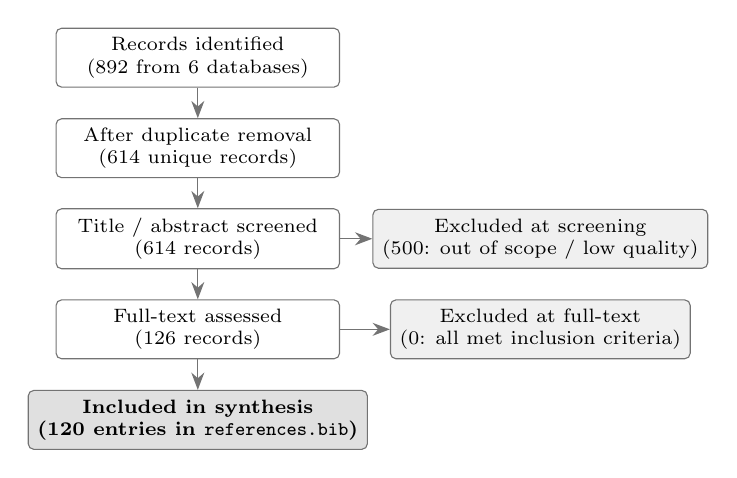
\begin{tikzpicture}[prisma/.style={draw=black!55, fill=white, rounded corners=2pt, minimum width=3.6cm, minimum height=0.72cm, align=center, font=\scriptsize}, prismaem/.style={prisma, fill=black!6, minimum width=3.0cm, minimum height=0.58cm}, arr/.style={-{Stealth[length=2.2mm]}, line width=0.45pt, draw=black!55}
]
  \node[prisma] (id) at (0,0) {Records identified\\(892 from 6 databases)};
  \node[prisma] (dedup) at (0,-1.15) {After duplicate removal\\(614 unique records)};
  \node[prisma] (screen) at (0,-2.3) {Title / abstract screened\\(614 records)};
  \node[prismaem] (excl1) at (4.35,-2.3) {Excluded at screening\\(500: out of scope / low quality)};
  \node[prisma] (full) at (0,-3.45) {Full-text assessed\\(126 records)};
  \node[prismaem] (excl2) at (4.35,-3.45) {Excluded at full-text\\(0: all met inclusion criteria)};
  \node[prisma, fill=black!12, font=\scriptsize\bfseries] (incl) at (0,-4.6)
    {Included in synthesis\\(120 entries in \texttt{references.bib})};
  \draw[arr] (id) -- (dedup);
  \draw[arr] (dedup) -- (screen);
  \draw[arr] (screen) -- (full);
  \draw[arr] (full) -- (incl);
  \draw[arr] (screen.east) -- (excl1.west);
  \draw[arr] (full.east) -- (excl2.west);
\end{tikzpicture}
\caption[PRISMA-style literature screening flow]{PRISMA-style literature screening flow}
\label{fig:prisma-flow}
\end{figure}

\begin{table}[H]
\centering
\footnotesize
\setlength{\tabcolsep}{4pt}
\renewcommand{\arraystretch}{1.12}
\caption[Top-10 ranked literature sources]{Top-10 ranked literature sources}
\label{tab:lit-top10}
\resizebox{\textwidth}{!}{%
\begin{tabular}{@{}cp{4.2cm}p{7.4cm}@{}}
\toprule
\tableheadcolor
\tableheadfont \# & \tableheadfont Source / Module / Operationalized In & \tableheadfont Headline Finding \\
\midrule
1 & Werner et al.\ 2022 [1] · DeFi mechanics · Ch.~3 & DeFi lending is uniformly flat, pool-based, overcollateralized \\
\rowcolor{RowShade}
2 & Tan 2023 (IMF) [5] · CBDC \& hierarchy · Ch.~3 & Two-tier CBDC distribution (central bank $\to$ commercial banks $\to$ users); hierarchical infrastructure is the key design choice \\
3 & Palaiokrassas et al.\ 2024 [3] · Fraud detection · Sec.~\ref{sec:aiml-support} & Multi-chain ML on 54M tx, F1 0.76--0.85 with behavioral features \\
\rowcolor{RowShade}
4 & Adom et al.\ 2022 [4] · Explainable AI · Sec.~\ref{sec:aiml-support} & SHAP outperforms LIME on lending datasets \\
5 & Weber et al.\ 2019 / Elliptic [85] · Graph fraud · Sec.~\ref{sec:gnn-extension} & Graph-structured fraud signal in BTC transactions \\
\rowcolor{RowShade}
6 & McMahan et al.\ 2017 / FedAvg [68] · Federated learning · Sec.~\ref{sec:fl-fraud} & Privacy-preserving model averaging across institutions \\
7 & BIS WP 905 [61] · Stablecoin risk · Secs.~\ref{sec:stablecoin-first}, \ref{sec:mica-compliance} & Algorithmic stablecoins unsuitable for EM DeFi; USDC/USDT recommended \\
\rowcolor{RowShade}
8 & Atzei et al.\ 2017 [7] · Smart contract security · Sec.~\ref{sec:defense-in-depth} & SoK of EVM attack vectors \\
9 & EU MiCA + GENIUS Act [75, 77] · Regulation · Sec.~\ref{sec:mica-compliance} & Stablecoin issuer authorization, reserve disclosure \\
\rowcolor{RowShade}
10 & Bangladesh Bank SP2025-02 [80] · MFI precedent · Sec.~\ref{sec:over-indebt} & Female-to-male account parity 49\%/49\% in 2025; 89\% BRAC loans to women \\
\bottomrule
\end{tabular}%
}
\end{table}

\section{Review of Existing Research}
\label{sec:review-existing}

This part of the paper explores all the literature chosen through a PRISMA-style screening flow to select the papers that best fit our project. We surveyed existing work related to DeFi lending, ML fraud detection and explainable AI, hierarchical development finance and cross-tier finance flows, group or microfinance, smart contracts and gas economics, retail banking and payments, remittance, monetary-policy distributional effects, real-world asset tokenization, stablecoin regulation and institutional settlement, and how inference can be achieved in systems like ours.

\subsection{Decentralized Lending and DeFi Protocol Design}

This is one of the most important parts of the paper: how decentralized financing works for lending, and how DeFi protocols are designed as public smart contracts. Utilization curves set interest rates; oracles trigger liquidations on collateral; settlement stays atomic across currencies. The model's real strength is real-time auditability---per-block interest and transparent on-chain state. It also comes with structural limits for development finance: capital still flows one way through flat pools, with no inter-tier allocation or multi-entity co-funding---a crucial gap for our project.

Werner et al.~[1] summarize DeFi as homogeneous, pool-based, and over-collateralized, with no institutional hierarchy. Bastankhah et al.~[2] show adaptive fast/slow rate control outperforming static Aave/Compound curves~[51], which informs our kinked-rate model (Section~\ref{sec:kinked-rate}). Chen et al.~[39] test multi-chain lending layouts to handle higher throughput. Yang and Cui~[40] propose practical metrics---utilization stability, liquidation efficiency, and rate responsiveness---for judging how well a lending stack performs. Hartmann and Hasan~[41] look at gas cost and digital identity in peer-to-peer lending. Dao et al.~[52] map traditional credit scoring onto DeFi borrowing limits.

\subsection{Machine Learning, Explainable AI, and Extended AI Security}

Palaiokrassas et al.~[3] achieve F1 0.76--0.85 on 54M multi-chain DeFi transactions using behavioral features versus 0.08 with raw transaction data alone---direct input to Random Forest feature engineering. Liu et al.~[6] supply Isolation Forest for unsupervised detection when labeled fraud is scarce. Hasan et al.~[42] train fraud classifiers via federated learning on encrypted features, informing cross-bank intelligence without raw data sharing.

Adom et al.~[4] find SHAP more consistent than LIME for loan explanations; Yuan~[49] reaches AUC $>$0.92 with SHAP on credit-default models---motivating SHAP waterfall review before approvals. Beyond the core pipeline, graph features from Palaiokrassas et al.~[3] support GNN ring detection; federated learning~[42] suits National/Local Bank boundaries; ContractWard~[43] and SoliAudit~[44] enable real-time exploit monitoring; RL rate tuning and NLP income extraction remain future-work options.

\subsection{Hierarchical Distribution, Cross-Tier Flows, and Group Lending}
\label{sec:lit-cross-tier}

Tan~[5] models two-tier CBDC distribution (central bank $\to$ commercial banks $\to$ users), paralleling the four-tier hierarchy. BIS~[46] prefers two-level retail CBDC with interoperability constraints, informing the dual-currency facility. Asaduzzaman et al.~[47] report up to 60\% admin-cost reduction from smart-contract microcredit---literature precedent for \texttt{GroupLendingPool}, not a deployment-jurisdiction claim.

Policy literature establishes hierarchical distribution but sparse programmable \emph{multi-directional} coordination. Kiff et al.~[106] distinguish multi-tier CBDC with supervised intermediaries; Bindseil~[105] analyses tiered remuneration for \texttt{UpwardDepositFacility} rate spreads (Section~\ref{sec:upward-flow}); Auer and B\"{o}hme~[107] hybrid CBDC mirrors client-via-Local-Bank access with Tier~1 reserve authority. \textit{Project Pine}~[103] validates layered contract factories for reserve and collateral dependencies extended by \texttt{InterBankLendingPool} and \texttt{SyndicatedLoan}. Dong et al.~[104] model cross-tier direct financing in supply chains---parallel to downward allocation to capital-constrained retail clients (Figure~\ref{fig:cross-tier-lending}).

Grameen/BRAC solidarity groups achieve $>$95\% repayment through social monitoring that on-chain mutual liability cannot fully replicate; \texttt{GroupLendingPool} encodes multi-signature consent and pool claims at pre-thesis stage. G\"{u}\c{c}\"uk et al.~[53] review privacy and trust in blockchain microlending.

\subsection{Smart Contract Security and Layer~2 Scalability}

Atzei et al.~[7] catalogue reentrancy, access-control, and overflow vectors---motivating OpenZeppelin guards, Solidity~0.8.20, RBAC, Slither, Mythril, and Phase~IV formal verification. Wang et al.~[43] (ContractWard) reach F1 0.96/0.93 on bytecode vulnerability classes; Liao et al.~[44] (SoliAudit) cut audit time $\approx$70\% via ML-prioritized fuzzing; So et al.~[45] (VERISMART) report 98.4\% precision with zero false positives on arithmetic safety---candidate for reserve-ratio invariants.

Kim and Kim~[48] show batching and calldata compression save 30--50\% mainnet gas, supporting Polygon zkEVM Cardona deployment where multi-step four-tier lifecycles multiply savings.

\subsection{Correspondent Banking, Retail Payments, and Settlement Rails}
\label{sec:lit-retail-payments}

BIS~[16] and FSB~[27] document nostro/vostro idle capital, MT103 routing, and 2--5-day settlement. World Bank remittance data~[20] average 6.49\% on a \$200 transfer (Sub-Saharan Africa $>$8\%). Cerutti et al.~[116] and Du et al.~[110] show digital and stablecoin rails can undercut legacy costs but depend on corridor off-ramp depth---scoped separately (Section~\ref{sec:future-retail-payments}).

Retail literature examines stablecoin remittance, merchant checkout, and on/off-ramps for post-MVT modules (\texttt{CurrentAccount}, \texttt{P2PTransfer}). Ante~[108] finds 26\% U.S.\ remittance-user stablecoin adoption, supporting tiered KYC gating. Du et al.~[110] document the fiat--stablecoin--fiat ``sandwich'' pattern. Li et al.~[109] (\textbf{CLEAR} framework) find programmable settlement advantages but weak open-loop dispute recourse; Zhang et al.~[112] warn on refund volatility; Fr\"{o}hlich et al.~[111] show on-ramp friction dominates POS UX. Lin et al.~[113] (\textit{SecurePay}) and BIS \textit{Project Sela}~[119] validate Local-Bank--sponsored multi-intermediary flows; Cimaszewski et al.~[118] blueprint jurisdictional DLT settlement. CPMI~[114], BIS Papers~170~[115], and FATF~[117] define ramp and VASP compliance for platform-mediated \texttt{P2PTransfer}---not permissionless unhosted-wallet remittance. No prior work composes four-tier development-finance lending with closed-loop retail rails in one architecture.

\subsection{Monetary Policy, Tokenization, and Institutional Landscape}
\label{sec:lit-institutional}

Cross-country evidence links QE to wealth inequality~[28]; Federal Reserve metro analysis~[29] shows low-income harm from tightening---motivating algorithmic, transparent rate and reserve parameters rather than opaque committee discretion. Tier-uniform utilization rates reduce loan-officer price discrimination; the Cantillon effect does not apply where USDC is fully reserved and the platform creates no new money~[30].

R3 Corda reports \$17B tokenized RWAs~[31]; Centrifuge exceeds \$1B across eight chains~[32]; World Bank FundsChain tracks disbursements on 13 projects scaling to 250~[33]---institutional precedent for hierarchical on-chain finance beyond fund tracking alone.

Sygnum~[65] notes institutional allocators require legal enforceability (Aave Arc $\approx$\$50k TVL). mBridge~[78] and \textit{Project Agora}~[79] are settlement rails, not retail lending hierarchies; 94\% of central banks research CBDCs~[71]. CWB positions as a lending-layer specification compatible with these rails.

\subsection{Graph ML, Federated Learning, Regulation, and Identity Primitives}

DeFi fraud is relational: Cheng et al.~[93], Chang et al.~[93], and DeFiGuard~[67] outperform flat ML on graph structure---motivating a GNN extension with hierarchical tier edges (Section~\ref{sec:gnn-extension}). Federated learning~[42, 97] and PrivChain-AI (94.7\% accuracy) suit banks that cannot share raw records; FedAvg aggregation at National tier is architecturally natural (Section~\ref{sec:fl-fraud}).

MiCA~[75, 76] and the U.S.\ GENIUS Act~[77] anchor stablecoin-first retail design (Section~\ref{sec:stablecoin-first}; mapping in Section~\ref{sec:mica-compliance}). Buterin et al.~[69] introduce non-transferable SBTs for portable credit passports~[70] (Section~\ref{sec:credit-passport}).

\subsection{Oracle-Mediated ML and Optional LLM Interfaces}
\label{sec:lit-llm}

Luo et al.~[94] survey AI fraud detection across the DeFi lifecycle; Caldarelli~[95] identifies ML-score oracle delivery as under-researched beyond price feeds. BCCC-DeFiFraudTrans-2025~[83] (1,026,867 labeled transactions) is the planned primary training corpus after pre-thesis 2 (Section~\ref{sec:ml-workload}); Fazliani et al.~[96] and Alhasawi et al.~[97] supply semi-supervised and federated baselines.

The optional conversational add-on uses an 8B open-weight LLM with QLoRA, RAG, and refusal layers. Finance LLM studies~[72, 73, 74] report productivity gains but document regulatory-hallucination risks---motivating the red-team protocol in Section~\ref{sec:llm-eval}.

\section{Literature Review Summary}

Tables~\ref{tab:lit-summary} and~\ref{tab:lit-summary-b} consolidate the reviewed works by methodology, findings, and project relevance. Extended six-part synthesis tables are maintained in the thesis repository~[17].

\begin{table}[H]
\centering
\footnotesize
\setlength{\tabcolsep}{3pt}
\renewcommand{\arraystretch}{1.08}
\caption[Literature review summary (Part 1 of 2)]{Literature review summary (Part 1 of 2)}
\label{tab:lit-summary}
\resizebox{\textwidth}{!}{%
\begin{tabular}{@{}>{\raggedright\arraybackslash}p{3.0cm}>{\raggedright\arraybackslash}p{2.6cm}>{\raggedright\arraybackslash}p{3.4cm}>{\raggedright\arraybackslash}p{3.2cm}@{}}
\toprule
\tableheadcolor
\tableheadfont Author \& Focus & \tableheadfont Methodology & \tableheadfont Key Findings & \tableheadfont Relevance to Our Project \\
\midrule
Palaiokrassas et al.\ (2024) [3] · DeFi fraud & XGBoost, NN on 54M+ txs & F1: 0.76--0.85 vs.\ 0.08 with features alone & Random Forest fraud modeling \\
Adom et al.\ (2022) [4] · XAI lending & LIME / SHAP comparison & SHAP deeper, more consistent than LIME & Primary explainability method \\
Tan (2023) [5] · CBDC hierarchy & Developing-nation model & Two-tier CBDC distribution; hierarchy decisive & Four-tier architecture \\
Liu et al.\ (2008) [6] · Anomaly detection & Isolation Forest & Recursive partitioning; shorter paths & Unsupervised wallet detection \\
Atzei et al.\ (2017) [7] · SC security & SoK of Ethereum attacks & Reentrancy, access-control gaps & Security primitives, formal verification \\
Werner et al.\ (2022) [1] · DeFi SoK & Survey of 12+ protocol types & Pool-based, overcollateralised; no hierarchy & Core gap CWB addresses \\
Bastankhah et al.\ (2024) [2] · Adaptive lending & Dual fast/slow control & Dynamic rates beat static curves & Kinked-rate validation \\
Hartmann \& Hasan (2021) [41] · P2P lending & Smart-contract origination & Gas minimisation; no intermediary & Four-tier P2P design \\
Hasan et al.\ (2022) [42] · Federated fraud & FL on encrypted features & Comparable to centralised ML & Cross-bank intelligence \\
Wang et al.\ (2020) [43] · SC vulnerabilities & ML on bytecode & F1: 0.96 access control; 0.93 leakage & Security verification models \\
Liao et al.\ (2019) [44] · Audit automation & Classification + fuzzing & 70\% faster than manual audit & Security audit strategy \\
\bottomrule
\end{tabular}%
}
\TableScreenshotEnd{Literature Review Summary (Part 1 of 2): DeFi, ML, and Security}
\end{table}

\begin{table}[H]
\centering
\footnotesize
\setlength{\tabcolsep}{3pt}
\renewcommand{\arraystretch}{1.08}
\caption[Literature review summary (Part 2 of 2)]{Literature review summary (Part 2 of 2)}
\label{tab:lit-summary-b}
\resizebox{\textwidth}{!}{%
\begin{tabular}{@{}>{\raggedright\arraybackslash}p{3.0cm}>{\raggedright\arraybackslash}p{2.6cm}>{\raggedright\arraybackslash}p{3.4cm}>{\raggedright\arraybackslash}p{3.2cm}@{}}
\toprule
\tableheadcolor
\tableheadfont Author \& Focus & \tableheadfont Methodology & \tableheadfont Key Findings & \tableheadfont Relevance to Our Project \\
\midrule
BIS et al.\ (2020) [46] · CBDC design & Retail distribution analysis & Two-tier preferred; interoperability gaps & Dual-currency facility \\
Kiff et al.\ (2020) [106] · CBDC models & IMF architecture survey & Multi-tier via supervised intermediaries & Wholesale-to-retail path \\
Bindseil (2020) [105] · CBDC rates & ECB tiered remuneration & Preserves bank intermediation & Asymmetric rate spread \\
Dong et al.\ (2023) [104] · Supply-chain finance & Three-tier game model & Cross-tier direct financing & Downward client lending \\
Project Pine (2025) [103] · Hierarchical SCs & NY Fed / BIS prototype & Factory-to-facility hierarchy & \texttt{IBLP} / \texttt{SyndicatedLoan} \\
BIS/FSB [16] · Cross-border settlement & Nostro/vostro cost analysis & 2--5 days; \$42/transfer avg. & Near-instant four-tier settlement \\
Beyer et al.\ (2025) [28] · QE inequality & Cross-country 1999--2019 & QE raises wealth inequality & Algorithmic monetary parameters \\
World Bank (2025) [33] · Dev.\ finance blockchain & 13-project pilot & Reduces reporting burden & Multi-chain deployment \\
Chen et al.\ (2024) [39] · Multi-chain lending & Cross-chain design & Higher throughput, less congestion & Multi-chain strategy \\
Yang \& Cui (2023) [40] · Protocol evaluation & Quantitative risk metrics & Utilisation, liquidation, responsiveness & Tier benchmarks \\
Asaduzzaman et al.\ (2020) [47] · Smart micro-credit & Smart-contract MFI & 60\% admin overhead reduction & \texttt{GroupLendingPool} \\
Kim \& Kim (2024) [48] · Gas optimisation & Batching, calldata compression & 30--50\% gas savings & L2 deployment \\
Yuan (2024) [49] · SHAP credit default & RF, GBM + SHAP & AUC $>$0.92, interpretable & Per-client risk explanation \\
\bottomrule
\end{tabular}%
}
\TableScreenshotEnd{Literature Review Summary (Part 2 of 2): Hierarchy, Institutions, and Retail Rails}
\end{table}

\newpage
\begin{table}[H]
\centering
\footnotesize
\setlength{\tabcolsep}{3pt}
\renewcommand{\arraystretch}{1.08}
\caption[]{Literature review summary (Part 2 of 2, continued)}
\resizebox{\textwidth}{!}{%
\begin{tabular}{@{}>{\raggedright\arraybackslash}p{3.0cm}>{\raggedright\arraybackslash}p{2.6cm}>{\raggedright\arraybackslash}p{3.4cm}>{\raggedright\arraybackslash}p{3.2cm}@{}}
\toprule
\tableheadcolor
\tableheadfont Author \& Focus & \tableheadfont Methodology & \tableheadfont Key Findings & \tableheadfont Relevance to Our Project \\
\midrule
Ante (2025) [108] · Stablecoin remittance & U.S.\ survey ($n{=}866$) & 26\% adoption; literacy drives uptake & KYC ladder, \texttt{P2PTransfer} \\
Du et al.\ (2026) [110] · Payment rails & Corridor cost comparison & Stablecoin sandwich undercuts banks & PSP on/off-ramp work \\
Li et al.\ (2026) [109] · Retail payments SoK & CLEAR framework & Closed-loop advantage; weak disputes & Merchant checkout design \\
Zhang et al.\ (2024) [112] · Stablecoin checkout & Operations model & Refund volatility disutility & \texttt{FXModule}, auto-conversion \\
Fr\"{o}hlich et al.\ (2022) [111] · Crypto POS & Lightning usability & On-ramp friction dominates & Fiat-funded \texttt{CurrentAccount} \\
Lin et al.\ (2025) [113] · Platform payments & Permissioned chain prototype & $\approx$256~TPS; multi-intermediary escrow & Local-Bank merchant flows \\
CPMI / BIS [114, 115] · Stablecoin policy & Cross-border analysis & Ramps gate acceptance & Ramp integration \\
FATF (2021) [117] · VASP / P2P & Risk-based AML & Platform transfers need originator data & Sponsored \texttt{P2PTransfer} \\
\bottomrule
\end{tabular}%
}
\end{table}

\section{Comparative Protocol Analysis}
\label{sec:comparative-protocol}

No surveyed protocol combines multi-tier hierarchy, oracle-mediated explainable ML, and compliance-aware identity. Table~\ref{tab:protocol-comparison} compares CWB against Aave, Compound, Maker, Maple, and Goldfinch on eleven architectural dimensions.

\begin{table}[H]
\centering
\footnotesize
\setlength{\tabcolsep}{3pt}
\resizebox{\textwidth}{!}{%
\begin{tabular}{@{}p{3.4cm}*{6}{>{\centering\arraybackslash}p{1.35cm}}@{}}
\toprule
\tableheadcolor
\tableheadfont Feature & \tableheadfont Aave & \tableheadfont Comp. & \tableheadfont Maker & \tableheadfont Maple & \tableheadfont Gfinch & \tableheadfont CWB \\
\midrule
Institutional hierarchy & \tmarkNo{} & \tmarkNo{} & \tmarkNo{} & \tmarkNo{} & \tmarkNo{} & \tmarkPlanned{} \\
\rowcolor{RowShade}
Cross-tier capital flow & \tmarkNo{} & \tmarkNo{} & \tmarkNo{} & \tmarkNo{} & \tmarkNo{} & \tmarkPartial{} \\
Same-tier interbank lending & \tmarkNo{} & \tmarkNo{} & \tmarkNo{} & \tmarkNo{} & \tmarkNo{} & \tmarkPartial{} \\
\rowcolor{RowShade}
Syndicated / co-lending & \tmarkNo{} & \tmarkNo{} & \tmarkNo{} & Part. & Part. & \tmarkPartial{} \\
Upward capital repatriation & \tmarkNo{} & \tmarkNo{} & \tmarkNo{} & \tmarkNo{} & \tmarkNo{} & \tmarkPartial{} \\
\rowcolor{RowShade}
Solidarity group lending & \tmarkNo{} & \tmarkNo{} & \tmarkNo{} & \tmarkNo{} & Part. & \tmarkPlanned{} \\
AI/ML fraud detection & \tmarkNo{} & \tmarkNo{} & \tmarkNo{} & Man. & Man. & \tmarkPlanned{} \\
\rowcolor{RowShade}
SHAP explainability & \tmarkNo{} & \tmarkNo{} & \tmarkNo{} & \tmarkNo{} & \tmarkNo{} & \tmarkPlanned{} \\
ZKP KYC compliance & \tmarkNo{} & \tmarkNo{} & \tmarkNo{} & \tmarkNo{} & \tmarkNo{} & \tmarkPlanned{} \\
\rowcolor{RowShade}
Kinked interest rate curve & \tmarkDone{} & \tmarkDone{} & Gov. & \tmarkDone{} & \tmarkNo{} & \tmarkPartial{} \\
Role-based access control & Part. & Part. & Gov. & \tmarkDone{} & Part. & \tmarkPlanned{} \\
\rowcolor{RowShade}
Institutional / L2 focus & \tmarkNo{} & \tmarkNo{} & \tmarkNo{} & \tmarkDone{} & Part. & \tmarkPlanned{} \\
TVL / Status (2026) & \$26B & \$1.4B & \$10B & \$2.6B & \$680M & Planning \\
\bottomrule
\end{tabular}%
}
\caption[Protocol comparison on eleven architectural dimensions]{Protocol comparison on eleven architectural dimensions}
\label{tab:protocol-comparison}
\end{table}

This answers RQ1: flat-pool protocols differentiate assets, not institutional relationships or inter-bank flows; Maple, Goldfinch, and Morpho~V2~[117, 90] lack multilateral development-finance capital allocation. CWB's compound novelty (Section~\ref{sec:research-contribution}) spans hierarchy, explainable ML governance, and group lending. Tiers~1--3 use bespoke RBAC (Section~\ref{sec:defense-in-depth}) functionally equivalent to ERC-3643 token-level KYC gating~[82]; enforced per-tier reserve ratios address opaque custody failures such as FTX's 2022 collapse.

Six design decisions follow from the survey:
\begin{itemize}[noitemsep]
\item Gudgeon et al.~[56] $\to$ kinked-rate model (Section~\ref{sec:kinked-rate})
\item Piper et al.~[58] $\to$ ZKP identity path (Section~\ref{sec:identity})
\item Tan~[5], BIS~[46], Kiff~[106], Auer and B\"{o}hme~[107] $\to$ four-tier capital flows
\item Bindseil~[105], Project Pine~[103], Dong et al.~[104] $\to$ multi-directional lending (Section~\ref{sec:cross-tier-lending})
\item Asaduzzaman et al.~[47] $\to$ \texttt{GroupLendingPool}
\item Ante~[108], Du et al.~[110], Li et al.~[109], Lin et al.~[113], CPMI~[114], FATF~[117] $\to$ post-MVT retail stack (Section~\ref{sec:future-retail-payments})
\end{itemize}

\section{Summary of Key Findings}
\label{sec:lit-key-findings}

The literature review yields the following design-relevant conclusions:

\begin{itemize}[noitemsep]
\item \textbf{Flat DeFi vs.\ tiered finance.} Pool-based protocols exceed \$55B TVL~[8] but lack institutional hierarchy; CBDC research confirms tiered distribution as a workable pattern~[5]. No prior work models four-tier reserve-enforced lending.
\item \textbf{Settlement and retail rails.} Correspondent banking traps idle capital~[18], settles in 2--5 days at $\approx$\$42/transfer~[19], and costs remittance users \$48--56B annually~[20]. Stablecoin rails can compress costs~[116, 110] but need ramp infrastructure; retail studies~[109, 112, 111, 113, 119] favour Local-Bank--sponsored closed-loop flows over open permissionless checkout.
\item \textbf{ML, XAI, and security.} Behavioral DeFi features lift fraud F1 to 0.76--0.85~[3]; Isolation Forest~[6] covers unlabeled cases; SHAP beats LIME for regulatory explainability~[4]. Contract vulnerabilities are well catalogued~[7]; ML audit tools reach F1 $>$0.93~[43], cut review time 70\%~[44], and formal verifiers such as VERISMART reach 98.4\% precision~[45].
\item \textbf{Hierarchy, groups, and institutions.} Cross-tier CBDC and Project Pine literature~[106, 105, 107, 103, 104] supports multi-directional programmable flows; analogue MFIs report $>$95\% group repayment~[47] with on-chain mutual liability still an open gap. FundsChain~[33], Corda RWAs~[31], and Kinexys~[34] show rising institutional blockchain adoption.
\item \textbf{Scalability, privacy, and regulation.} Multi-chain lending~[39] and L2 gas optimization~[48] cut costs 30--50\%; federated learning~[42, 97] enables cross-bank fraud intelligence without raw data sharing. MiCA and GENIUS~[75, 77] anchor stablecoin-first design; algorithmic parameters mitigate distributional opacity from discretionary monetary policy~[28, 29].
\item \textbf{Deposit-funded sustainability.} Sustainable MFIs rely on mobilized deposits, not donor capital alone---motivating savings vaults at the Local Bank tier alongside \texttt{GroupLendingPool}.
\end{itemize}

These findings justify the four-tier architecture, cross-tier lending modules, Random Forest / Isolation Forest / SHAP analytics, governance structure, and phased security verification pipeline developed in later chapters.

%% CHAPTER 3 (compressed): architecture essentials only
\chapter{System Architecture and Design}
\label{ch:architecture-compressed}

This chapter compresses Chapter~3 of \texttt{Pre-thesis\_v31\_final.tex} to the architecture an examiner needs at pre-thesis~1: scope, tiers, contracts, data partition, oracle path, and security framing. All architecture diagrams from the full thesis are included in Section~\ref{sec:architecture-figures}.

\section{Prototype Scope and Stack}
\label{sec:prototype-scope}

Four Agile phases (I--IV) deliver a four-tier EVM lending stack on \textbf{Polygon zkEVM Cardona} with \textbf{Solidity~0.8.20}, \textbf{React + Wagmi} frontend, \textbf{PostgreSQL + FastAPI} off-chain services, and \textbf{Chainlink} for prices, automation, ML-score delivery, and proof-of-reserve. Table~\ref{tab:prototype-scope} lists build status; most on-chain modules are \textit{specified} now and deploy in Phases~II--IV.

\begin{table}[H]
\centering
\caption[Prototype scope (summary)]{Prototype scope (summary)}
\label{tab:prototype-scope}
\footnotesize
\begin{tabular}{@{}p{7.2cm}>{\raggedleft\arraybackslash}p{5.5cm}@{}}
\toprule
\tableheadcolor
\tableheadfont Feature & \tableheadfont Status \\
\midrule
Four-tier RBAC (World / National / Local / Client) & Specified (Phase~I) \\
Loan lifecycle + installments & Specified / Phase~II \\
SavingsVault, GroupLendingPool, IBLP & Specified / Phase~II \\
RF + IF + SHAP oracle pipeline & Planned (Phase~III) \\
ZKP KYC, testnet deploy, Foundry sim & Planned (Phase~IV) \\
Optional MCP agent (17 tools) & Optional (Phase~III--IV) \\
\bottomrule
\end{tabular}
\end{table}

\section{High-Level Architecture}
\label{sec:high-level-arch}

\textbf{Four layers:} (1)~React wallet UI; (2)~Express/FastAPI APIs and ML scorer; (3)~15 modular Solidity contracts across Tier~1--3; (4)~Polygon zkEVM + Chainlink oracles. Tier~1 \texttt{WorldBankReserve} custodies reserves and allocates downward; Tier~2 \texttt{NationalBank}; Tier~3 \texttt{LocalBank} runs retail loans, KYC gates, and installments; Tier~4 clients hold Credit Passport SBTs and borrowing limits.

\textbf{Core contracts (Phase~I--II):} \texttt{WorldBankReserve}, \texttt{NationalBank}, \texttt{LocalBank}, \texttt{SavingsVault}, \texttt{FixedDeposit}, \texttt{GroupLendingPool}, \texttt{FXModule}, \texttt{InsuranceFund}, \texttt{CurrentAccount}, \texttt{InterBankLendingPool}, \texttt{UpwardDepositFacility}, \texttt{TreasurySwap}. \textbf{Phase~III stretch:} \texttt{SyndicatedLoan}, \texttt{TranchedPool}, \texttt{NettingEngine}.

\section{Oracle and ML Integration}
\label{sec:oracle-architecture}
\label{sec:ml-explainability}
\label{sec:aiml-support}

Off-chain Random Forest + Isolation Forest produce a composite risk score~$s$; SHAP explains declines. Scores reach \texttt{LoanController} via \textbf{Chainlink Functions} (primary) or a \textbf{commit-reveal} relay (prototype). Approval is blocked until \texttt{SCORE\_REVEALED}. Chainlink Automation triggers overdue installments; Price Feeds support \texttt{FXModule}.

\section{Data Model and Partitioning}
\label{sec:data-model-compressed}

Twenty PostgreSQL entities (3NF) mirror on-chain loan state, installments, market data, ML audit logs, and optional agent sessions. \textbf{On-chain:} balances, roles, loan state machine, reserve ratios, committed scores. \textbf{Off-chain:} PII, SHAP JSON, chat history, indexed events. Identity uses zk-SNARK KYC (specified) + non-transferable Credit Passport SBT.

\section{Cross-Tier Operations and Products}
\label{sec:multi-entity}
\label{sec:over-indebt}
\label{sec:interbank-pool}
\label{sec:bridge}
\label{sec:kinked-rate}
\label{sec:upward-flow}
\label{sec:credit-passport}
\label{sec:identity}

Capital moves \textbf{downward} (allocation), \textbf{same-tier} (interbank pools), and \textbf{upward} (surplus deposits). Group lending encodes solidarity consent; syndication handles large co-funded loans. Retail products: savings, fixed deposits, installment loans, FX display, insurance buffer.

\section{System Modeling and Security}
\label{sec:defense-in-depth}

Use-case, activity, DFD, sequence, and capital-flow diagrams model nine actor types and the USDC loan lifecycle. Security follows five layers: wallet/RBAC, contract guards (OpenZeppelin), oracle trust boundaries, API hardening (EIP-712), and operational monitoring. Threat model maps reentrancy, oracle manipulation, and privilege escalation to controls.


\section{Architecture Diagrams (Full Set)}
\label{sec:architecture-figures}

\begin{figure}[H]
\centering
\BalancedDiagram{fig-three-layer-arch.pdf}
\caption[Four-layer application architecture]{Four-layer application architecture}
\label{fig:three-layer-arch}
\end{figure}

\begin{figure}[H]
\centering
\BalancedDiagram{fig-component-architecture.pdf}
\caption[Component diagram (planning phase)]{Component diagram (planning phase)}
\label{fig:component-diagram}
\end{figure}

\begin{figure}[H]
\centering
\BalancedDiagram{fig-blockchain-stack.pdf}
\caption[Layered blockchain and application stack]{Layered blockchain and application stack}
\label{fig:blockchain-stack}
\end{figure}

\begin{figure}[H]
\centering
\BalancedDiagram{fig-oracle-architecture.pdf}
\caption[Chainlink oracle architecture]{Chainlink oracle architecture}
\label{fig:oracle-architecture}
\end{figure}

\begin{figure}[H]
\centering
\BalancedDiagram{fig-erd-core.pdf}
\caption[Core system entity graph]{Core system entity graph}
\label{fig:core-system-graph}
\end{figure}

\begin{figure}[H]
\centering
\BalancedDiagram{fig-erd-extended.pdf}
\caption[Extended ERD entities]{Extended ERD entities}
\label{fig:erd-extended}
\end{figure}

\begin{figure}[H]
\centering
\BalancedDiagram{fig-eer-model.pdf}
\caption[Enhanced EER model]{Enhanced EER model}
\label{fig:eer}
\end{figure}

\begin{figure}[H]
\centering
\BalancedDiagram{fig-data-partitioning.pdf}
\caption[On-chain versus off-chain data partitioning]{On-chain versus off-chain data partitioning}
\label{fig:data-partitioning}
\end{figure}

\begin{figure}[H]
\centering
\BalancedDiagram{fig-compliance-identity.pdf}
\caption[Compliance and identity stack]{Compliance and identity stack}
\label{fig:compliance-identity}
\end{figure}

\begin{figure}[H]
\centering
\ThesisIncludeGraphics[width=0.9\linewidth, keepaspectratio]{Ch3_actor-permission-matrix.pdf}
\caption[Actor permission matrix (primary actions)]{Actor permission matrix (primary actions)}
\label{fig:permission-matrix}
\end{figure}

\begin{figure}[H]
\centering
\BalancedDiagram{fig-tier-model.pdf}
\caption[Client limits and bank-level syndication]{Client limits and bank-level syndication}
\label{fig:tier-model}
\end{figure}

\begin{figure}[H]
\centering
\BalancedDiagram{fig-five-stage-funnel.pdf}
\caption[Five-stage retail onboarding funnel]{Five-stage retail onboarding funnel}
\label{fig:five-stage-funnel}
\end{figure}

\begin{figure}[H]
\centering
\BalancedDiagram{fig-agent-six-step-pipeline.pdf}
\caption[Optional AI agent add-on (Phase III--IV, excluded from MVT)]{Optional AI agent add-on (Phase III--IV, excluded from MVT)}
\label{fig:agent-six-step-pipeline}
\end{figure}

\begin{figure}[H]
\centering
\HalfWidthDiagram{fig-kinked-rate-curve.pdf}
\caption[Kinked utilization-based borrowing rate]{Kinked utilization-based borrowing rate}
\label{fig:kinked-rate-curve}
\end{figure}

\begin{figure}[H]
\centering
\HalfWidthDiagram{fig-liquidation-engine.pdf}
\caption[LiquidationEngine tier models and lifecycle]{LiquidationEngine tier models and lifecycle}
\label{fig:liquidation-engine}
\end{figure}

\begin{figure}[H]
\centering
\ThesisIncludeGraphics[width=0.9\linewidth, keepaspectratio]{fig-savings-vault.pdf}
\caption[SavingsVault and FixedDeposit closed loop]{SavingsVault and FixedDeposit closed loop}
\label{fig:savings-vault}
\end{figure}

\begin{figure}[H]
\centering
\HalfWidthDiagram{fig-credit-passport.pdf}
\caption[On-chain Credit Passport SBT lifecycle]{On-chain Credit Passport SBT lifecycle}
\label{fig:credit-passport}
\end{figure}

\begin{figure}[H]
\centering
\BalancedDiagram{fig-ccip-bridge.pdf}
\caption[Chainlink CCIP cross-chain hierarchy invariant]{Chainlink CCIP cross-chain hierarchy invariant}
\label{fig:ccip-bridge}
\end{figure}

\begin{figure}[H]
\centering
\BalancedDiagram{Ch3_multi-entity-cross-tier-operations.pdf}
\caption[Multi-entity and cross-tier capital operations]{Multi-entity and cross-tier capital operations}
\label{fig:multi-entity-ops}
\end{figure}

\begin{figure}[H]
\centering
\BalancedDiagram[width=0.98\linewidth]{Ch3_use-case-nine-actor-taxonomy.pdf}
\caption[Use-case diagram (nine-actor taxonomy)]{Use-case diagram (nine-actor taxonomy)}
\label{fig:usecase}
\end{figure}

\begin{figure}[H]
\centering
\ActivityDiagram{fig-activity-lending.pdf}
\caption[USDC loan lifecycle activity flow]{USDC loan lifecycle activity flow}
\label{fig:act-lending}
\label{fig:act-loan}\label{fig:act-hierarchy}
\end{figure}

\begin{figure}[H]
\centering
\ActivityDiagram{fig-activity-onboarding-id.pdf}
\caption[Retail onboarding and identity activity flow]{Retail onboarding and identity activity flow}
\label{fig:act-onboarding}
\label{fig:act-income}\label{fig:act-profile}
\end{figure}

\begin{figure}[H]
\centering
\ActivityDiagram{fig-activity-aux.pdf}
\caption[Client banking session activity flow]{Client banking session activity flow}
\label{fig:act-aux}
\label{fig:act-chat}\label{fig:act-aichatbot}\label{fig:act-market}
\end{figure}

\begin{figure}[H]
\centering
\BalancedDiagram{Ch3_data-flow-diagrams.pdf}
\caption[Data-flow diagrams]{Data-flow diagrams}
\label{fig:dfd-suite}
\label{fig:dfd-context}\label{fig:dfd-level1a}\label{fig:dfd-level1b}
\end{figure}

\begin{figure}[H]
\centering
\BalancedDiagram{fig-seq-loan-flow.pdf}
\caption[Loan approval sequence diagram]{Loan approval sequence diagram}
\label{fig:seq-loan-flow}
\label{fig:seq-loan}\label{fig:seq-reject}
\end{figure}

\begin{figure}[H]
\centering
\BalancedDiagram{fig-seq-installment-income.pdf}
\caption[Sequence diagrams]{Sequence diagrams}
\label{fig:seq-installment-income}
\label{fig:seq-installment}\label{fig:seq-income}
\end{figure}

\begin{figure}[H]
\centering
\BalancedDiagram{fig-seq-banking-data.pdf}
\caption[Sequence diagrams]{Sequence diagrams}
\label{fig:seq-banking-data}
\label{fig:seq-hierarchy}\label{fig:seq-marketdata}\label{fig:seq-borrowlimit}
\end{figure}

\begin{figure}[H]
\centering
\BalancedDiagram{fig-seq-chat-chatbot.pdf}
\caption[Sequence diagrams]{Sequence diagrams}
\label{fig:seq-chat-bot}
\label{fig:seq-chat}\label{fig:seq-aichatbot}
\end{figure}

\begin{figure}[H]
\centering
\BalancedDiagram{fig-hierarchical-banking.pdf}
\caption[Four-tier hierarchical capital flow]{Four-tier hierarchical capital flow}
\label{fig:four-tier}
\end{figure}

\begin{figure}[H]
\centering
\BalancedDiagram{fig-governance-dual-path.pdf}
\caption[Governance dual-path]{Governance dual-path}
\label{fig:governance-dual-path}
\end{figure}

\begin{figure}[H]
\centering
\BalancedDiagram{fig-sar-aml-workflow.pdf}
\caption[SAR and AML compliance workflow]{SAR and AML compliance workflow}
\label{fig:sar-aml-workflow}
\end{figure}

\begin{figure}[H]
\centering
\BalancedDiagram{fig-defense-in-depth.pdf}
\caption[Five-layer defense-in-depth security architecture]{Five-layer defense-in-depth security architecture}
\label{fig:defense-in-depth}
\end{figure}

\begin{figure}[H]
\centering
\BalancedDiagram{fig-security-controls.pdf}
\caption[Smart-contract security controls]{Smart-contract security controls}
\label{fig:security-controls}
\end{figure}
%% CHAPTER 4 (compressed): methodology summary
\chapter{Methodology}
\label{ch:methodology-compressed}

Lightweight \textbf{Agile/Scrum} across four implementation phases. \textbf{Core thesis} = on-chain banking + oracle ML; conversational agent is optional (Could-have).

\section{MVT Checklist and Phase Plan}
\label{sec:mvt-checklist}

Graded pass line: (C1) four-tier contracts on testnet; (C2) \texttt{GroupLendingPool} spec + PoC; (C3) RF/IF/SHAP + Authority Brief after pre-thesis~2. Pre-thesis~1 delivers specification only---no trained models or live deploy.

\begin{table}[H]
\centering
\caption[Four-phase implementation summary]{Four-phase implementation summary}
\label{tab:phase-summary}
\begin{tabular}{p{1.4cm}p{3.8cm}p{1.6cm}p{6.5cm}}
\toprule
\tableheadcolor
\textbf{Phase} & \textbf{Focus} & \textbf{Weeks} & \textbf{Key deliverables} \\
\midrule
I & Foundation & 1--4 & Contract hierarchy, DB schema, React shell \\
II & Core banking & 5--9 & Loan E2E, savings, group pool, automation \\
III & ML + oracle & 10--13 & Chainlink Functions, Authority Brief, dashboard \\
IV & Verification & 14--16 & Foundry sim, Certora stretch, testnet manifest \\
\bottomrule
\end{tabular}
\end{table}

\begin{table}[H]
\centering
\caption[Core vs.\ optional capabilities]{Core vs.\ optional capabilities}
\label{tab:capability-priority}
\begin{tabular}{p{3.2cm}p{2.2cm}p{7.8cm}}
\toprule
\tableheadcolor
\textbf{Capability} & \textbf{Priority} & \textbf{Phase / interface} \\
\midrule
Four-tier smart contracts & Must (I--II) & React + wallet; Foundry tests \\
On-chain loan lifecycle & Must (II) & \texttt{LoanController} state machine \\
Chainlink Functions oracle & Must (III) & FastAPI $\to$ DON $\to$ on-chain score \\
RF + IF + SHAP & Must (III) & Authority Brief; audit log \\
MCP conversational agent & Could (III--IV) & Alternate API path only \\
\bottomrule
\end{tabular}
\end{table}

\section{Design Decisions}
\label{sec:design-decisions}
\label{sec:gnn-extension}
\label{sec:fl-fraud}
\label{sec:ml-workload}

\begin{table}[H]
\centering
\caption[Design decisions (selected)]{Design decisions (selected)}
\label{tab:design-decisions}
\footnotesize
\begin{tabular}{p{2.8cm}p{2.6cm}p{2.6cm}p{4.5cm}}
\toprule
\tableheadcolor
\textbf{Area} & \textbf{Choice} & \textbf{Alternative} & \textbf{Criterion} \\
\midrule
Network & Polygon zkEVM Cardona & Amoy PoS & ZK validity proofs, low gas \\
Contracts & Solidity EVM & Solana & Tooling, testnet cost \\
Fraud ML & Random Forest + IF & XGBoost & SHAP compatibility \\
Oracle & Chainlink Functions & Commit-reveal only & Decentralised trust \\
Database & PostgreSQL & SQLite & 3NF, async API \\
\bottomrule
\end{tabular}
\end{table}


\section{Methodology Diagrams (Full Set)}
\label{sec:methodology-figures}
\label{sec:llm-eval}
\label{sec:future-retail-payments}

\begin{figure}[H]
\centering
\BalancedDiagram{fig-agile-process.pdf}
\caption[Agile / Scrum development process]{Agile / Scrum development process}
\label{fig:agile-process}
\end{figure}

\begin{figure}[H]
\centering
\BalancedDiagram{fig-aiml-pipeline.pdf}
\caption[AI/ML pipeline wiring]{AI/ML pipeline wiring}
\label{fig:aiml-pipeline}
\end{figure}

\begin{figure}[H]
\centering
\small
\begin{minipage}[t]{0.48\linewidth}
\centering
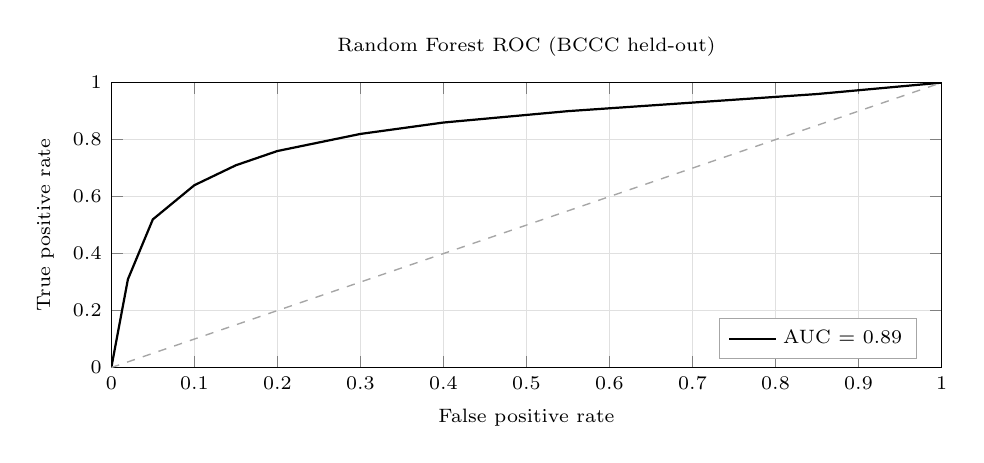
\begin{tikzpicture}
\begin{axis}[
 width=\linewidth,
 height=5.2cm,
 xlabel={False positive rate},
 ylabel={True positive rate},
 xmin=0, xmax=1,
 ymin=0, ymax=1,
 grid=both,
 grid style={black!12},
 tick label style={font=\scriptsize},
 label style={font=\scriptsize},
 title={\scriptsize Random Forest ROC (BCCC held-out)},
 title style={font=\scriptsize},
 legend style={font=\scriptsize, at={(0.97,0.03)}, anchor=south east, draw=black!35, fill=white},
]
\addplot[black, line width=0.8pt, mark=none]
 coordinates {
 (0,0) (0.02,0.31) (0.05,0.52) (0.10,0.64) (0.15,0.71)
 (0.20,0.76) (0.30,0.82) (0.40,0.86) (0.55,0.90) (0.70,0.93)
 (0.85,0.96) (1,1)
 };
\addlegendentry{AUC = 0.89}
\addplot[black!35, dashed, line width=0.5pt] coordinates {(0,0) (1,1)};
\end{axis}
\end{tikzpicture}

\vspace{4pt}
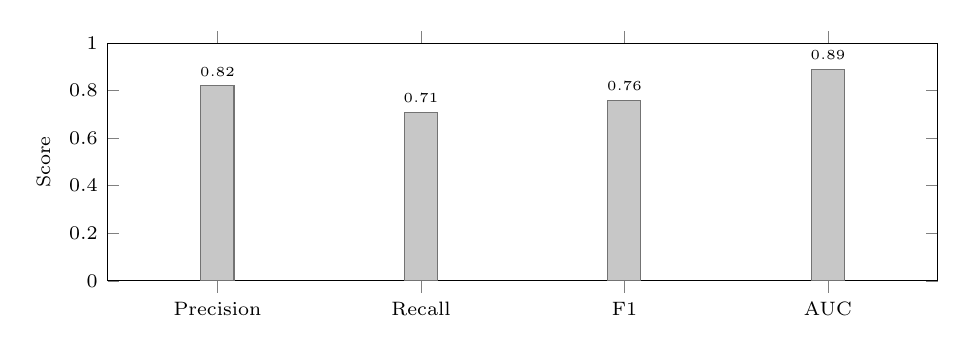
\begin{tikzpicture}
\begin{axis}[
 width=\linewidth,
 height=4.6cm,
 ybar,
 bar width=0.42cm,
 symbolic x coords={Precision, Recall, F1, AUC},
 xtick=data,
 ymin=0, ymax=1,
 ylabel={Score},
 tick label style={font=\scriptsize},
 label style={font=\scriptsize},
 nodes near coords={\pgfmathprintnumber[fixed, precision=2]{\pgfplotspointmeta}},
 every node near coord/.append style={font=\tiny},
 enlarge x limits=0.18,
]
\addplot[fill=black!22, draw=black!55] coordinates {
 (Precision, 0.82) (Recall, 0.71) (F1, 0.76) (AUC, 0.89)
};
\end{axis}
\end{tikzpicture}
\end{minipage}\hfill
\begin{minipage}[t]{0.48\linewidth}
\centering
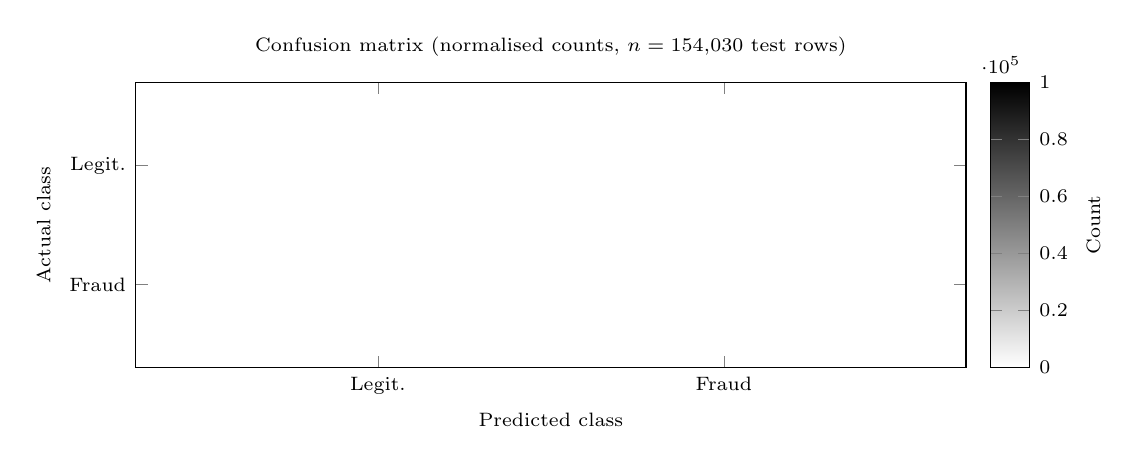
\begin{tikzpicture}
\begin{axis}[width=\linewidth, height=5.2cm, xlabel={Predicted class}, ylabel={Actual class}, xtick={0, 1}, ytick={0, 1}, xticklabels={Legit., Fraud}, yticklabels={Legit., Fraud}, tick label style={font=\scriptsize}, label style={font=\scriptsize}, title={\scriptsize Confusion matrix (normalised counts, $n=154{, }030$ test rows)}, title style={font=\scriptsize}, colorbar, colormap={greyscale}{color(0cm)=(white); color(1cm)=(black!)}, point meta min=0, point meta max=100000, colorbar style={font=\scriptsize, ylabel={Count}}, ]
\addplot[matrix plot, mesh/cols=2, mesh/rows=2, shader=flat corner, ] table[meta=z] {
 x y z
 0 0 98420
 1 0 1180
 0 1 820
 1 1 610
};
\end{axis}
\end{tikzpicture}

\vspace{4pt}
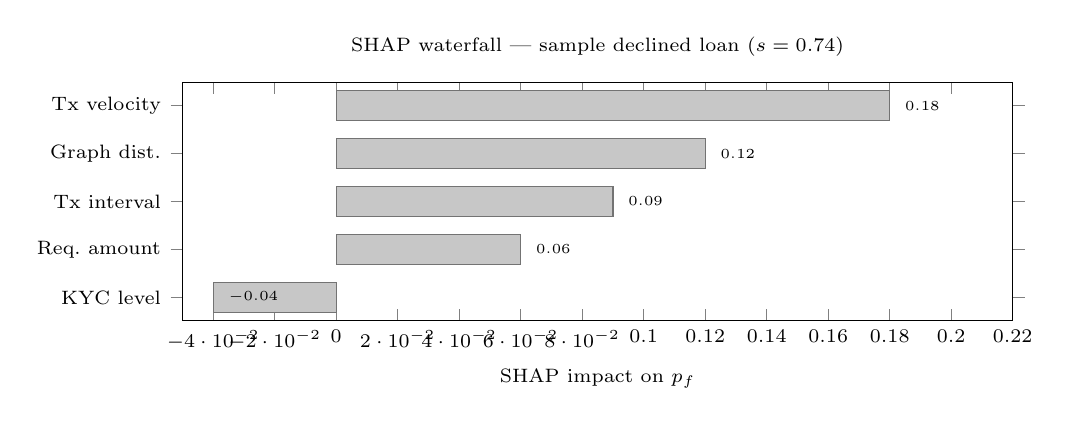
\begin{tikzpicture}
\begin{axis}[
 width=\linewidth,
 height=4.6cm,
 xbar,
 bar width=0.38cm,
 xmin=-0.05, xmax=0.22,
 symbolic y coords={%
 KYC level, Req.\ amount, Tx interval, Graph dist., Tx velocity%
 },
 ytick=data,
 xlabel={SHAP impact on $p_f$},
 tick label style={font=\scriptsize},
 label style={font=\scriptsize},
 title={\scriptsize SHAP waterfall --- sample declined loan ($s=0.74$)},
 title style={font=\scriptsize},
 nodes near coords={\pgfmathprintnumber[fixed, precision=2]{\pgfplotspointmeta}},
 every node near coord/.append style={font=\tiny, anchor=west, xshift=2pt},
 enlarge y limits=0.12,
]
\addplot[fill=black!22, draw=black!55] coordinates {
 (0.18,Tx velocity) (0.12,Graph dist.) (0.09,Tx interval)
 (0.06,Req.\ amount) (-0.04,KYC level)
};
\end{axis}
\end{tikzpicture}
\end{minipage}
\caption[Planned ML evaluation layout (post pre-thesis 2)]{Planned ML evaluation layout (post pre-thesis 2)}
\label{fig:ml-eval}
\end{figure}

\begin{figure}[H]
\centering
\BalancedDiagram{fig-ml-explainability.pdf}
\caption[Explainability and anomaly-detection flow]{Explainability and anomaly-detection flow}
\label{fig:ml-explainability}
\end{figure}

\begin{figure}[H]
\centering
\ActivityDiagram{fig-realtime-dashboard.pdf}
\caption[Real-time dashboard and runtime monitoring pipeline]{Real-time dashboard and runtime monitoring pipeline}
\label{fig:realtime-dashboard}
\end{figure}

\begin{figure}[H]
\centering
\BalancedDiagram{Ch4_loan-lifecycle-state-machine.pdf}
\caption[Transaction state machine of the loan lifecycle]{Transaction state machine of the loan lifecycle}
\label{fig:tx-state-machine}
\end{figure}

\begin{figure}[H]
\centering
\ActivityDiagram{Ch4_four-phase-roadmap-sdlc.pdf}
\caption[Four-phase roadmap with SDLC mapping and progress]{Four-phase roadmap with SDLC mapping and progress}
\label{fig:phase-roadmap}
\end{figure}

\begin{figure}[H]
\centering
\HalfWidthDiagram{fig-phase-effort-bar.pdf}
\caption[Development effort by implementation phase]{Development effort by implementation phase}
\label{fig:phase-effort}
\end{figure}

\begin{figure}[H]
\centering
\ThesisIncludeGraphics[width=0.75\linewidth, height=0.54\textheight, keepaspectratio]{fig-optional-agent-addon.pdf}
\caption[Optional conversational agent add-on]{Optional conversational agent add-on}
\label{fig:optional-agent-addon}
\end{figure}

\begin{figure}[H]
\centering
\ActivityDiagram{Ch4_dev-verification-toolchain.pdf}
\caption[Planned development and verification toolchain]{Planned development and verification toolchain}
\label{fig:dev-toolchain}
\end{figure}

\begin{figure}[H]
\centering
\BalancedDiagram{Ch4_design-decisions-alternatives.pdf}
\caption[Key design decisions and alternatives considered]{Key design decisions and alternatives considered}
\label{fig:design-decisions}
\end{figure}
%% ---------------------------------------------------------------------------
%% CHAPTER 5 --- SHORT VERSION AUTHORING NOTES (mirrored in chapterinstruction box)
%% Keep: perf eval (1 para), design analysis (1 para), final adjustments (1 para),
%% four feasibility tables, statistical tables + 2 figures (planning projections only),
%% market/customer/partner tables (NOT Ch.2 protocol-comparison duplicate), discussion limits.
%% Target ~8--12 pages. Full source: Pre-thesis_v31_final.tex lines 2972--3257.
%% ---------------------------------------------------------------------------
%% CHAPTER 5 (compressed)
\chapter{Evaluation and Discussion}
\label{ch:evaluation-compressed}

\begin{chapterinstruction}{Authoring instructions --- Chapter 5 (short version)}
\textbf{Goal:} Show feasibility ``slightly'' for pre-thesis~1; label all numbers as \textit{planning projections} until pre-thesis~2 evidence exists.

\textbf{Must include (in order):}
\begin{enumerate}[noitemsep]
\item \textbf{Performance evaluation} (1 short paragraph): pre-thesis~1 = specs only; live gas/ML benchmarks deferred to pre-thesis~2; point to MVT checklist.
\item \textbf{Analysis of design solutions} (1 paragraph): justify stack (zkEVM L2, Solidity, PostgreSQL, Chainlink Functions); optional agent outside MVT.
\item \textbf{Final design adjustment} (1 paragraph): four locks --- stablecoin-first, L2 gas, ML as decision-support only, MVT scope boundary.
\item \textbf{Feasibility analysis} --- keep all \textbf{four tables}: technical, economic (\$0 prototype), risk taxonomy, regulatory/MiCA mapping.
\item \textbf{Statistical analysis} --- keep revenue-assumption table, ETH-sensitivity table, default-scenario table, and both APR/revenue figures; open with ``planning projections, not observed data.''
\item \textbf{Comparisons and relationships} --- keep market-sizing, customer-segment, and partner-role tables; \textbf{do not} duplicate the Ch.~2 protocol-comparison table.
\item \textbf{Discussion} (1 short section): five explicit limitations (compound novelty, BCCC baseline, testnet scope, group lending $\neq$ BRAC, oracle drift).
\end{enumerate}

\textbf{Cut from full Ch.~5:} long prose repeats, duplicate competitor table, appendix-level detail. Target: $\approx$8--12 pages with tables + 2 figures.
\end{chapterinstruction}

\section{Performance Evaluation}
\label{sec:performance-eval}
\label{sec:cost-model}
\label{sec:gas-cost}
\label{sec:eval-method}

Pre-thesis~1 delivers specifications and planned checks, not live benchmarks. Component and economic feasibility are in Section~\ref{sec:feasibility}; RQ-level evaluation follows Section~\ref{sec:eval-method} after pre-thesis~2 (testnet deployment, gas measurement, ML metrics, MVT demo). On L2, projected gas per loan stays below interest earned; default stress is in Table~\ref{tab:default-scenarios}.

\section{Analysis of Design Solutions}
\label{sec:design-solutions-ch5}

Stack choices were scored on ecosystem maturity, zero-cost prototype constraints, and auditability (Table~\ref{tab:design-decisions}, Section~\ref{sec:design-decisions}). The selected path pairs EVM Solidity on zkEVM L2, PostgreSQL + FastAPI off-chain, and Chainlink Functions (with commit-reveal as an interim relay) for ML scores. The optional MCP agent and EIP-7702 session keys remain Phase~III--IV extensions outside the MVT.

\section{Final Design Adjustment}
\label{sec:final-design-adjustment}

The final pre-thesis design locks four adjustments before implementation: (i)~\textbf{stablecoin-first} retail lending (USDC/USDT, Section~\ref{sec:stablecoin-first}) to avoid ETH liability volatility; (ii)~\textbf{L2 deployment} for micro-loan gas economics; (iii)~\textbf{ML as decision support only}---human approvers and on-chain gates, no auto-disbursement; (iv)~\textbf{MVT scope} limited to the three-tier lending core, database schema, and dashboard---syndicated/tranched modules, full regulatory filing, and the conversational agent are deferred (Table~\ref{tab:mvt-checklist}).

\section{Feasibility Analysis}
\label{sec:feasibility}

\subsection{Technical Feasibility}

Each layer is specified against mature tooling; nothing requires bespoke infrastructure beyond standard testnets and open-source stacks (Table~\ref{tab:tech-feasibility}).

\begin{table}[H]
\centering
\caption[Technical feasibility assessment]{Technical feasibility assessment}
\label{tab:tech-feasibility}
\begin{tabular}{p{3cm}p{3cm}p{7.5cm}}
\toprule
\tableheadcolor
\textbf{Component} & \textbf{Assessment} & \textbf{Evidence} \\
\midrule
Smart contracts & Feasible (specified) & Solidity; Hardhat; OpenZeppelin; Phases~I--II \\
Frontend DApp & Feasible (specified) & React~18 + Wagmi/RainbowKit \\
Blockchain deployment & Feasible (planned) & Polygon zkEVM Cardona + Sepolia \\
AI/ML integration & Feasible with constraints & RF + IF + SHAP; Chainlink Functions Phase~III \\
Optional agent & Feasible (deferred) & MCP + Qwen3-8B; Phase~III--IV; outside MVT \\
Database backend & Feasible & PostgreSQL 20-entity schema (3NF); FastAPI \\
\bottomrule
\end{tabular}
\end{table}

\vspace{2pt}

\subsection{Economic Feasibility}

The academic prototype can run at \textbf{zero direct cost}; scaled hosting is a separate pilot concern (Table~\ref{tab:economic-feasibility}). L2 gas keeps small loans viable versus mainnet; spread revenue and default scenarios are modelled in Section~\ref{sec:statistical-analysis}.

\begin{table}[H]
\centering
\caption[Economic feasibility --- zero-cost prototype]{Economic feasibility --- zero-cost prototype}
\label{tab:economic-feasibility}
\begin{tabular}{p{4cm}p{2.5cm}p{7cm}}
\toprule
\tableheadcolor
\textbf{Cost Category} & \textbf{Estimate} & \textbf{Notes} \\
\midrule
Blockchain deployment & \$0 & Public testnets \\
Frontend / backend hosting & \$0 & Vercel / Render free tiers or localhost \\
AI/ML training & \$0 & Local machine or Colab free tier \\
Development tools & \$0 & Hardhat, VS Code, Git (open-source) \\
\textbf{Total prototype} & \textbf{\$0} & Pilot ops $\approx$\$500--\$2{,}000/month at scale \\
\bottomrule
\end{tabular}
\end{table}

\vspace{2pt}

\subsection{Risk Feasibility}

Main delivery risks and mitigations are summarised in Table~\ref{tab:risk-taxonomy}; smart-contract and regulatory items dominate severity.

\begin{table}[H]
\centering
\caption[Risk taxonomy and mitigation]{Risk taxonomy and mitigation}
\label{tab:risk-taxonomy}
\begin{tabular}{p{3cm}p{4cm}p{1.5cm}p{5cm}}
\toprule
\tableheadcolor
\textbf{Risk Category} & \textbf{Description} & \textbf{Severity} & \textbf{Mitigation} \\
\midrule
Partner non-cooperation & Key partners decline to join & Medium & Testnet pilots; open-source replication \\
Smart contract vulnerability & Logic exploit & High & OpenZeppelin; audits; pause mechanism \\
Regulatory adversity & Jurisdiction blocks retail crypto & Medium & Testnet-only prototype; sandbox path \\
AI/ML model degradation & Fraud model drift & Low & Retraining; human-in-the-loop; SHAP review \\
\bottomrule
\end{tabular}
\end{table}

\vspace{2pt}

\subsection{Regulatory Feasibility}
\label{sec:mica-compliance}

Retail stablecoin lending must align with MiCA, GENIUS Act, and EU AI Act expectations; CWB uses authorised stablecoins and keeps PII off-chain (Table~\ref{tab:mica-mapping}). Full conformity files and national licensing remain future work; pre-thesis scope is testnet demonstration only.

\begin{table}[H]
\centering
\caption[Regulatory design controls (selected)]{Regulatory design controls (selected)}
\label{tab:mica-mapping}
\begin{tabular}{p{3.2cm}p{4.6cm}p{5.8cm}}
\toprule
\tableheadcolor
\textbf{Statute / Article} & \textbf{Requirement} & \textbf{CWB Control} \\
\midrule
MiCA Art.~16 & Authorised EMT issuer & Uses USDC/USDT; does not issue \\
MiCA Art.~36 & 1{:}1 reserve backing & Issuer attestations before pool acceptance \\
EU AI Act (credit scoring) & High-risk AI from Aug.~2026~ & Human approver gate; SHAP + audit log \\
GDPR Art.~17 & Right to erasure & PII off-chain only; hashes on-chain \\
\bottomrule
\end{tabular}
\end{table}

\section{Statistical Analysis}
\label{sec:statistical-analysis}
\label{sec:interest-rates}

The tables below model spread revenue, ETH-price sensitivity, and default stress at full-deployment scale (planning assumptions only; not observed platform data). Interest tiers follow the 3\%/5\%/8\% hierarchy (Figure~\ref{fig:apr-spread}).

\begin{table}[H]
\centering
\caption[Revenue projection assumptions]{Revenue projection assumptions}
\label{tab:revenue-assumptions}
\begin{tabular}{p{6cm}p{7.5cm}}
\toprule
\tableheadcolor
\textbf{Parameter} & \textbf{Value} \\
\midrule
Reference ETH price & \$2{,}500 (planning mid-point, Feb 2026) \\
World Bank $\to$ National Bank & 3\% APR \\
National Bank $\to$ Local Bank & 5\% APR \\
Local Bank $\to$ Client & 8\% APR \\
Average loan term & 12 months \\
Default rate provision (base) & 8\% \\
Origination fee & 0.25\% per disbursement \\
\bottomrule
\end{tabular}
\end{table}

\vspace{2pt}

\begin{table}[H]
\centering
\caption[ETH-price sensitivity of spread revenue]{ETH-price sensitivity of spread revenue}
\begin{tabular}{@{}lccc@{}}
\toprule
\tableheadcolor
\tableheadfont ETH Price & \tableheadfont Loan Base & \tableheadfont Spread Revenue & \tableheadfont Incl.\ Fees (est.) \\
\midrule
\$2{,}000 & \$1.376B & \$110.1M & \$120--128M \\
\rowcolor{RowShade}
\$2{,}500 (base) & \$1.720B & \$137.6M & \$150--159M \\
\$3{,}000 & \$2.064B & \$165.1M & \$180--191M \\
\bottomrule
\end{tabular}
\end{table}

\vspace{2pt}

\begin{table}[H]
\centering
\caption[Default-rate sensitivity]{Default-rate sensitivity}
\label{tab:default-scenarios}
\begin{tabular}{@{}lccp{4.8cm}@{}}
\toprule
\tableheadcolor
\tableheadfont Scenario & \tableheadfont Default rate & \tableheadfont Annual loss & \tableheadfont Basis \\
\midrule
Optimistic & 3.7\% & \$7.4M & Mature MFI benchmarks~ \\
\rowcolor{RowShade}
Base case & 8\% & \$16M & New platform, limited history \\
Stress & 15\% & \$30M & Thin credit history, volatile collateral \\
\bottomrule
\end{tabular}
\end{table}

\begin{figure}[H]
\centering
\HalfWidthDiagram{fig-revenue-by-tier.pdf}
\caption[Annual revenue projection (10-year maturity)]{Annual revenue projection (10-year maturity)}
\label{fig:revenue-by-tier}
\end{figure}

\begin{figure}[H]
\centering
\HalfWidthDiagram{fig-apr-spread.pdf}
\caption[Hierarchical interest-rate spread (APR)]{Hierarchical interest-rate spread (APR)}
\label{fig:apr-spread}
\end{figure}

\section{Comparisons and Relationships}
\label{sec:comparisons-relationships}

\begin{table}[H]
\centering
\caption[Market segments with supporting data]{Market segments with supporting data}
\label{tab:market-sizing-ch5}
\begin{tabular}{p{3.5cm}p{6.5cm}p{3cm}}
\toprule
\tableheadcolor
\textbf{Segment} & \textbf{Description} & \textbf{Estimated Scale} \\
\midrule
TAM & Global DeFi lending; remittances; MSME gap~[8, 15, 20] & \$55B -- 5T+ \\
SAM & Institutional hierarchical lending; emerging-market credit & \$5B -- 15B \\
SOM & Testnet pilots; sandbox partnerships & \$50 -- 200M \\
\bottomrule
\end{tabular}
\end{table}

\vspace{2pt}

\begin{table}[H]
\centering
\caption[Target customer segment profile]{Target customer segment profile}
\label{tab:customer-segment-ch5}
\begin{tabular}{p{3.5cm}p{10cm}}
\toprule
\tableheadcolor
\textbf{Characteristic} & \textbf{Description} \\
\midrule
Primary users & Tier~1--3 bank operators; Tier~4 retail via Local Banks \\
Loan range & Micro/SME at Local Bank tier; larger exposures via syndication \\
Key pain points & Opaque reserves; flat DeFi pools; weak explainability in on-chain lending \\
\bottomrule
\end{tabular}
\end{table}

\vspace{2pt}

\begin{table}[H]
\centering
\caption[Partner categories and roles]{Partner categories and roles}
\label{tab:partner-categories-ch5}
\begin{tabular}{p{3.5cm}p{4.5cm}p{5.5cm}}
\toprule
\tableheadcolor
\textbf{Partner Category} & \textbf{Role} & \textbf{Incentive} \\
\midrule
Financial regulators & Sandbox oversight & On-chain audit trails \\
Banking institutions & National/Local Bank nodes & Reserve access; lower settlement friction \\
Oracle providers & Chainlink DON, indexing & Unified oracle stack \\
Academic partners & ML / formal-verification review & Datasets; co-publication \\
\bottomrule
\end{tabular}
\end{table}

\vspace{2pt}

Market, customer, and partner tables below complement the protocol comparison in Chapter~2 (Table~\ref{tab:protocol-comparison}).

\section{Discussion}
\label{sec:ch5-discussion}
\label{sec:research-limitations}
\label{sec:bangladesh-reg}

This pre-thesis specifies architecture and planned evaluation; deployment evidence, trained models, and formal proofs arrive after pre-thesis~2. Five examiner-facing limits are recorded explicitly:

\begin{itemize}[noitemsep]
\item \textbf{Novelty is compound, not absolute}---Maple, Goldfinch, and Morpho cover parts of institutional credit; the claim is the four-tier reserve stack plus explainable oracle ML plus group liability in one open design.
\item \textbf{BCCC is a baseline only}---flat-pool fraud labels may not transfer to hierarchical CWB flows without testnet retraining.
\item \textbf{Testnet scope}---workshop-grade evidence needs benchmarks and reproducible repos; MVT deployment supplies the empirical layer.
\item \textbf{Group lending}---on-chain cosigning is not social solidarity; BRAC/Grameen statistics inform design only.
\item \textbf{Oracle and economics}---scores attach at origination; collusion and model drift remain open; Certora proofs state assumptions explicitly.
\end{itemize}

The prototype runs on public testnets with test tokens only. Jurisdiction-specific pilots (e.g.\ regulatory sandboxes) are future work; the architecture is global L2 institutional DeFi, not a single-country rollout claim.

%% ---------------------------------------------------------------------------
%% CHAPTER 6 --- SHORT VERSION AUTHORING NOTES (mirrored in chapterinstruction box)
%% Keep: opening problem (1 para), banking grounding (1 para), C1--C4 bullets,
%% institutional positioning (1 para), pre-thesis status (1 para).
%% Future work: 1 para or <=6 bullets. Cut long retail/regulatory essays.
%% Full source: Pre-thesis_v31_final.tex lines 3261--3313.
%% ---------------------------------------------------------------------------
\chapter{Conclusion}

\begin{chapterinstruction}{Authoring instructions --- Chapter 6 (short version)}
\textbf{Goal:} Close the thesis in 2--4 pages; restate contributions without re-explaining architecture.

\textbf{Must include:}
\begin{enumerate}[noitemsep]
\item \textbf{Opening} (1 paragraph): problem --- flat DeFi vs.\ hierarchical development finance; four-tier proposal in one sentence.
\item \textbf{Banking grounding} (1 paragraph): six banking functions encoded on-chain; multi-entity co-lending (solidarity + syndication) as differentiator.
\item \textbf{Four contributions} (bullet list): C1 four-tier architecture; C2 group lending; C3 explainable oracle ML; C4 ZKP identity --- each one line with honest built-vs-specified scope.
\item \textbf{Positioning} (1 paragraph): vs.\ institutional DeFi literature and MiCA/GENIUS regulatory frontier; no single competitor has full stack.
\item \textbf{Pre-thesis status} (1 paragraph): what this report delivers now vs.\ what MVT adds after pre-thesis~2.
\end{enumerate}

\textbf{Future work (compress to 1 paragraph or 6 bullets max):} hierarchical lending E2E, stablecoin deploy, deposit/group products, ML oracle live, simulation/Certora; optionally one line each on retail rails and GNN/FL research.

\textbf{Cut from full Ch.~6:} repeating Ch.~3--5 detail, long Future Work subsections (retail banking essay, regulatory deep-dive). Keep tone declarative, not promotional.
\end{chapterinstruction}

The \textit{Crypto World Bank} specifies a \textbf{four-tier institutional lending architecture} on EVM L2 that flat DeFi protocols (\$55B+ TVL) do not model: reserve-enforced capital flows from World Bank reserve to retail clients, with same-tier interbank pools, upward surplus deposits, and solidarity group lending.

\textbf{Contributions (scoped):} (C1)~hierarchical lending + multi-entity contracts; (C2)~programmable group liability; (C3)~oracle-mediated explainable ML; (C4)~privacy-preserving KYC path. The platform encodes six banking functions as auditable on-chain rules rather than discretionary enforcement.

\textbf{Pre-thesis~1 deliverable:} full architecture, literature, methodology, and feasibility framing; \textbf{after pre-thesis~2:} Cardona deploy, E2E loan demo, trained RF/IF on BCCC, populated MVT evidence. Future work: retail payment rails, GNN/federated extensions, Certora proofs, and regulatory pilots.

%% REFERENCES
\chapter*{References}
\phantomsection
\addcontentsline{toc}{chapter}{References}

{\small
\begin{enumerate}[label={[\arabic*]}]
\item S.~M. Werner, D.~Perez, L.~Gudgeon, A.~Klages-Mundt, D.~Harz, and W.~J. Knottenbelt, ``SoK: Decentralized Finance (DeFi),'' \textit{arXiv preprint arXiv:2101.08778}, 2022. [Online]. Available: \url{https://arxiv.org/abs/2101.08778}

\item M.~Bastankhah, V.~Nadkarni, C.~Jin, S.~Kulkarni, and P.~Viswanath, ``Thinking Fast and Slow: Data-Driven Adaptive DeFi Borrow-Lending Protocol,'' in \textit{Proc. 6th Conf. Advances in Financial Technologies (AFT)}, LIPIcs, vol.~316, pp.~27:1--27:23, 2024. DOI: \url{https://doi.org/10.4230/LIPIcs.AFT.2024.27}

\item G.~Palaiokrassas, S.~Scherrers, I.~Ofeidis, and L.~Tassiulas, ``Leveraging Machine Learning for Multichain DeFi Fraud Detection,'' in \textit{Proc. IEEE Int. Conf. Blockchain and Cryptocurrency (ICBC)}, 2024. DOI: \url{https://doi.org/10.1109/ICBC59979.2024.10634350}

\item D.~Adom, E.~O. Acheampong, and M.~Boateng, ``LIME and SHAP: A Comparison of Model-Agnostic Approaches to Explainability in Loan Approval Systems,'' \textit{International Journal of Advanced Computer Science and Applications}, vol.~13, no.~11, 2022.

\item B.~W. Tan, ``Central Bank Digital Currency and Financial Inclusion,'' \textit{IMF Working Paper WP/23/69}, 2023. [Online]. Available: \url{https://www.imf.org/en/Publications/WP/Issues/2023/03/27/Central-Bank-Digital-Currency-and-Financial-Inclusion-531273}. Accessed: June~9, 2026.

\item F.~T. Liu, K.~M. Ting, and Z.-H. Zhou, ``Isolation Forest,'' in \textit{Proc. IEEE Int. Conf. Data Mining (ICDM)}, pp.~413--422, 2008. DOI: \url{https://doi.org/10.1109/ICDM.2008.17}

\item N.~Atzei, M.~Bartoletti, and T.~Cimoli, ``A Survey of Attacks on Ethereum Smart Contracts (SoK),'' in \textit{Proc. Int. Conf. Principles of Security and Trust (POST)}, pp.~164--186, 2017. DOI: \url{https://doi.org/10.1007/978-3-662-54455-6_8}

\item DefiLlama, ``Lending Protocols --- DeFi TVL and Protocol Rankings,'' 2024--2026. [Online]. Available: \url{https://defillama.com/protocols/Lending}. Accessed: June~9, 2026.

\item World Bank, ``The Global Findex Database 2021: Financial Inclusion, Digital Payments, and Resilience,'' 2021. [Online]. Available: \url{https://www.worldbank.org/en/publication/globalfindex}. Accessed: June~9, 2026.

\item Aave, ``Aave Protocol Documentation,'' 2024. [Online]. Available: \url{https://docs.aave.com/}. Accessed: June~9, 2026.

\item Compound, ``Compound Protocol Documentation,'' 2024. [Online]. Available: \url{https://docs.compound.finance/}. Accessed: June~9, 2026.

\item BCOLBD 2025, ``Blockchain Olympiad Bangladesh: Guideline and Evaluation Scheme,'' 2025. [Online]. Available: \url{https://bcolbd.org/rules}. Accessed: June~9, 2026.

\item Galaxy Digital, ``The State of Crypto Lending and Borrowing,'' Galaxy Research, 2024. [Online]. Available: \url{https://www.galaxy.com/insights/research/the-state-of-crypto-lending}. Accessed: June~9, 2026.

\item World Bank, ``World Development Report 2022: Finance for an Equitable Recovery,'' 2022. [Online]. Available: \url{https://www.worldbank.org/en/publication/wdr2022}. Accessed: June~9, 2026.

\item International Finance Corporation (IFC), ``MSME Finance Gap: Assessment of the Shortfalls and Opportunities in Financing Micro, Small, and Medium Enterprises in Emerging Markets,'' World Bank, 2017. [Online]. Available: \url{https://openknowledge.worldbank.org/entities/publication/ff4c9839-21ac-5676-a23a-7cf6f745df0c}. Accessed: June~9, 2026.

\item Bank for International Settlements, ``DeFi Lending: Intermediation Without Information?,'' BIS Working Paper No.~1183, 2024. [Online]. Available: \url{https://www.bis.org/publ/work1183.pdf}. Accessed: June~9, 2026.

\item Michigan State University Libraries, ``Literature Table and Synthesis --- Nursing Literature Reviews,'' LibGuides, 2025. [Online]. Available: \url{https://libguides.lib.msu.edu/nursinglitreview/table}. Accessed: June~9, 2026.

\item Committee on Payments and Market Infrastructures and Bank for International Settlements, ``Correspondent Banking --- Technical Report,'' CPMI Papers No.~147, 2016. [Online]. Available: \url{https://www.bis.org/cpmi/publ/d147.pdf}. Accessed: June~9, 2026.

\item Ripple Labs, ``RLUSD Stablecoin Product Overview,'' Ripple Documentation, 2025. [Online]. Available: \url{https://ripple.com/solutions/stablecoin/}. Accessed: June~9, 2026.

\item World Bank, ``Remittance Prices Worldwide: Making Markets More Transparent,'' Migration and Development Brief~40, 2024. [Online]. Available: \url{https://remittanceprices.worldbank.org/}. Accessed: June~9, 2026.

\item DefiLlama, ``Aave V3 TVL, Fees, Revenue \& Income Statement,'' March 2026. [Online]. Available: \url{https://defillama.com/protocol/aave-v3}. Accessed: June~9, 2026.

\item World Inequality Lab, ``Exorbitant Privilege,'' \textit{World Inequality Report 2026}, 2026. [Online]. Available: \url{https://wir2026.wid.world/insight/exorbitant-privilege/}. Accessed: June~9, 2026.

\item DefiLlama, ``Compound V3 TVL, Fees, Revenue \& Income Statement,'' March 2026. [Online]. Available: \url{https://defillama.com/protocol/compound-v3}. Accessed: June~9, 2026.

\item Fensory, ``Sky Protocol Projects \$611M Revenue in 2026 as USDS Supply Targets \$20.6 Billion,'' February 2026. [Online]. Available: \url{https://www.fensory.com/intelligence/rwa/sky-protocol-tokenization-regatta-solana-february-2026}. Accessed: June~9, 2026.

\item Fensory, ``Maple Finance --- Institutional DeFi Lending Protocol,'' 2026. [Online]. Available: \url{https://www.fensory.com/insights/protocols/maple-finance}. Accessed: June~9, 2026.

\item Fensory, ``DeFi Credit Platforms Hit \$2.4B Milestone,'' March 2026. [Online]. Available: \url{https://www.fensory.com/intelligence/rwa/defi-private-credit-platforms-2-4-billion-loans-ethereum}. Accessed: June~9, 2026.

\item Financial Stability Board, ``Enhancing Cross-border Payments: Stage 3 Roadmap,'' 2020. [Online]. Available: \url{https://www.fsb.org/2020/10/enhancing-cross-border-payments-stage-3-roadmap/}. Accessed: June~9, 2026.

\item A.~Beyer, B.~Gasperini, and P.~Theodoridis, ``Monetary Policy and Inequality: Distributional Effects of Asset Purchase Programs,'' \textit{Journal of International Money and Finance}, vol.~157, 2025.

\item Federal Reserve Board, ``Monetary Policy and the Distribution of Income: Evidence from U.S. Metropolitan Areas,'' FEDS Notes, March 2025. [Online]. Available: \url{https://www.federalreserve.gov/econres/notes/feds-notes/monetary-policy-and-the-distribution-of-income-evidence-from-us-metropolitan-areas-20250331.html}. Accessed: June~9, 2026.

\item R.~Cantillon, \textit{Essai sur la Nature du Commerce en G\'en\'eral} (\textit{Essay on the Nature of Commerce in General}), 1755 (posthumous).

\item GlobeNewswire, ``R3's Corda Leads Tokenized RWA Market with Over \$10 Billion in On-chain Assets,'' February 2025. [Online]. Available: \url{https://www.globenewswire.com/news-release/2025/02/13/3025637/0/en/R3-s-Corda-leads-tokenized-RWA-market-with-over-10-billion-in-on-chain-assets-and-unrivalled-industry-adoption.html}. Accessed: June~9, 2026.

\item Centrifuge, ``Real-World Asset Tokenization: Key Trends from 2025,'' 2025. [Online]. Available: \url{https://centrifuge.io/blog/real-world-asset-tokenization-trends-2025}. Accessed: June~9, 2026.

\item World Bank, ``World Bank Group Tracks Project Funds with New Blockchain Tool,'' Press Release, September 2025. [Online]. Available: \url{https://www.worldbank.org/en/news/press-release/2025/09/26/world-bank-group-tracks-project-funds-with-new-blockchain-tool}. Accessed: June~9, 2026.

\item JPMorgan, ``Kinexys Digital Payments: Real-Time Multicurrency Payments,'' 2025. [Online]. Available: \url{https://www.jpmorgan.com/onyx/coin-system.htm}. Accessed: June~9, 2026.

\item World Economic Forum, ``Why Decentralized Finance Is a Leapfrog Technology for the 1.1 Billion People Who Are Unbanked,'' September 2022. [Online]. Available: \url{https://www.weforum.org/stories/2022/09/decentralized-finance-a-leapfrog-technology-for-the-unbanked/}. Accessed: June~9, 2026.

\item Opera Newsroom, ``160M CELO Allocation Proposal to Grow Opera from Distribution Partner into Key Network Stakeholder,'' March 2026. [Online]. Available: \url{https://press.opera.com/2026/03/19/opera-celo-partnership-2026/}. Accessed: June~9, 2026.

\item Morpho, ``Network Data,'' March 2026. [Online]. Available: \url{https://data.morpho.org/}. Accessed: June~9, 2026.

\item Stellar, ``End of Year 2025 Report --- Execution at Scale,'' 2025. [Online]. Available: \url{https://www.stellar.org/blog/foundation-news/2025-year-in-review}. Accessed: June~9, 2026.

\item Y.~Chen, S.~Bin, and H.~He, ``Design and Implementation of a Multi-Chain Lending Model in Blockchain,'' in \textit{Proc. 3rd Int. Conf. Artificial Intelligence and Computer Information Technology (AICIT)}, 2024, pp.~97--102.

\item S.~Yang and W.~Cui, ``An Evaluation System for DeFi Lending Protocols,'' \textit{arXiv preprint arXiv:2303.01022}, 2023. [Online]. Available: \url{https://arxiv.org/abs/2303.01022}

\item J.~Hartmann and O.~Hasan, ``A Social-Capital Based Approach to Blockchain-Enabled Peer-to-Peer Lending,'' in \textit{Proc. IEEE Int. Conf. Blockchain Computing and Applications (BCCA)}, pp.~105--110, 2021. [Online]. Available: \url{https://hal.science/hal-03371872}. Accessed: June~9, 2026.

\item P.~T.~Hasan, H.~K.~T.~Akhter, M.~R.~Tahsinur, A.~B.~Haque, A.~K.~M.~N.~Islam, and R.~M.~Rahman, ``Blockchain and Machine Learning for Fraud Detection: A Privacy-Preserving and Adaptive Incentive Based Approach,'' \textit{IEEE Access}, vol.~10, pp.~87115--87131, 2022. [Online]. Available: \url{https://ieeexplore.ieee.org/document/9857827}. Accessed: June~9, 2026.

\item Y.~Wang, J.~Liu, and Z.~Chen, ``ContractWard: Automated Vulnerability Detection Models for Ethereum Smart Contracts,'' \textit{IEEE Trans. Network Science and Engineering}, vol.~8, no.~2, pp.~1133--1144, 2020. DOI: \url{https://doi.org/10.1109/TNSE.2020.2968505}

\item C.-F.~Liao, T.-H.~Tsai, and C.-J.~Chen, ``SoliAudit: Smart Contract Vulnerability Assessment Based on Machine Learning and Fuzz Testing,'' in \textit{Proc. IEEE Int. Conf. Internet of Things (iThings)}, pp.~458--465, 2019. DOI: \url{https://doi.org/10.1109/iThings/GreenCom/CPSCom/SmartData.2019.00098}

\item S.~So, M.~Lee, J.~Park, H.~Lee, and H.~Oh, ``VERISMART: A Highly Precise Safety Verifier for Ethereum Smart Contracts,'' in \textit{Proc. IEEE Symp. Security and Privacy (S\&P)}, pp.~1678--1694, 2020. DOI: \url{https://doi.org/10.1109/SP40000.2020.00032}

\item Bank for International Settlements et al., ``Central Bank Digital Currencies: Foundational Principles and Core Features,'' BIS and Central Banks Joint Report, 2020. [Online]. Available: \url{https://www.bis.org/publ/othp33.htm}. Accessed: June~9, 2026.

\item M.~Asaduzzaman, F.~Hasib, and Z.~B.~Hafiz, ``Towards Using Blockchain Technology for Microcredit Industry in Bangladesh,'' in \textit{Proc. 23rd Int. Conf. Computer and Information Technology (ICCIT)}, pp.~1--6, 2020. DOI: \url{https://doi.org/10.1109/ICCIT51783.2020.9392730}

\item H.~Kim and D.~Kim, ``Optimal Gas Fee Minimization in DeFi: Enhancing Efficiency and Security on the Ethereum Blockchain,'' \textit{IEEE Access}, vol.~12, pp.~173810--173823, 2024. [Online]. Available: \url{https://ieeexplore.ieee.org/document/10750187}. Accessed: June~9, 2026.

\item X.~Yuan, ``SHAP-based Interpretable Models for Credit Default Assessment Using Machine Learning,'' in \textit{Proc. 14th Int. Conf. Software Technology and Engineering (ICSTE)}, pp.~213--217, 2024. DOI: \url{https://doi.org/10.1109/ICSTE63875.2024.00044}

\item G.~Wood, ``Ethereum: A Secure Decentralised Generalised Transaction Ledger'' (Yellow Paper), Ethereum Foundation, 2014 (revised 2023). [Online]. Available: \url{https://ethereum.github.io/yellowpaper/paper.pdf}. Accessed: June~9, 2026.

\item Aave, ``Aave Protocol V3 Technical Paper,'' 2022. [Online]. Available: \url{https://github.com/aave/aave-v3-core/blob/master/techpaper/Aave_V3_Technical_Paper.pdf}. Accessed: June~9, 2026.

\item T.~Dao, T.~Trinh, and V.~Pham, ``Optimizing Credit Scoring Models for Decentralized Financial Applications,'' in \textit{Information and Communication Technology}, Springer, 2025. DOI: \url{https://doi.org/10.1007/978-981-96-4282-3_36}

\item G.-L.~G\"{u}c\"{u}k, S.~Leible, and J.~Edinger, ``Blockchain-Based Microlending for Financial Inclusivity: A Literature Review of Its Privacy and Trust,'' Springer, 2024. DOI: \url{https://doi.org/10.1007/978-3-032-12801-0_22}

\item A.~Beniiche, ``A Study of Blockchain Oracles,'' \textit{arXiv preprint arXiv:2004.07140}, 2020. [Online]. Available: \url{https://arxiv.org/pdf/2004.07140}

\item A.~Pasdar, Y.~C.~Lee, and Z.~Dong, ``Connect API with Blockchain: A Survey on Blockchain Oracle Implementation,'' \textit{ACM Computing Surveys}, vol.~55, no.~10, 2023. DOI: \url{https://doi.org/10.1145/3567582}

\item L.~Gudgeon, S.~M.~Werner, D.~Perez, and W.~J.~Knottenbelt, ``DeFi Protocols for Loanable Funds: Interest Rates, Liquidity and Market Efficiency,'' in \textit{Proc. 2nd ACM Conf. Advances in Financial Technologies (AFT)}, pp.~92--112, 2020. DOI: \url{https://doi.org/10.1145/3419614.3423254}

\item K.~W.~Wu, ``Strengthening DeFi Security: A Static Analysis Approach to Flash Loan Vulnerabilities,'' \textit{arXiv preprint arXiv:2411.01230}, 2024.

\item F.~Piper, K.~Wolf, and J.~Heiss, ``Privacy-Preserving On-chain Permissioning for KYC-Compliant Decentralized Applications,'' TU Berlin, \textit{arXiv preprint arXiv:2510.05807}, 2025.

\item N.~Decker, ``Zero-Knowledge Proofs: Cryptographic Model for Financial Compliance and Global Banking Security,'' \textit{SSRN Working Paper No.~5170068}, 2025.

\item A.~Carstens et al., ``Stablecoins: Risks, Potential and Regulation,'' \textit{BIS Working Papers No.~905}, Bank for International Settlements, 2021. [Online]. Available: \url{https://www.bis.org/publ/work905.pdf}. Accessed: June~9, 2026.

\item ``Stablecoin Devaluation Risk,'' \textit{The European Journal of Finance}, Taylor \& Francis, 2025. DOI: \url{https://doi.org/10.1080/1351847X.2025.2505757}

\item J.~A.~Ocampo and K.~Gallagher, ``The Role of Multilateral Development Banks and Development Assistance in the Provision of Global Public Goods,'' UNDP Background Paper, 2024. [Online]. Available: \url{https://hdr.undp.org/system/files/documents/background-paper-document/2024jaocampokdgonzaleztheroleofmultilateraldevlmntbanks.pdf}. Accessed: June~9, 2026.

\item F.~A.~Aponte-Novoa, A.~L.~S.~Orozco, R.~Villanueva-Polanco, and P.~Wightman, ``The 51\% Attack on Blockchains: A Mining Behavior Study,'' \textit{IEEE Access}, vol.~9, pp.~140549--140564, 2021. DOI: \url{https://doi.org/10.1109/ACCESS.2021.3119291}

\item W3C, ``Decentralized Identifiers (DIDs) v1.0 --- Core Architecture, Data Model, and Representations,'' W3C Recommendation, July 2022. [Online]. Available: \url{https://www.w3.org/TR/did-core/}. Accessed: June~9, 2026.; see also W3C, ``Verifiable Credentials Data Model v1.1,'' W3C Recommendation, March 2022. [Online]. Available: \url{https://www.w3.org/TR/vc-data-model/}. Accessed: June~9, 2026.

\item Sygnum Bank, ``Institutional DeFi in 2025: From Niche to Mainstream Finance,'' Sygnum Research Report, February 2026. [Online]. Available: \url{https://www.sygnum.com/research/}. Accessed: June~9, 2026.

\item M.~J.~Page, J.~E.~McKenzie, P.~M.~Bossuyt, I.~Boutron, T.~C.~Hoffmann, C.~D.~Mulrow, et~al., ``The PRISMA 2020 statement: an updated guideline for reporting systematic reviews,'' \textit{BMJ}, vol.~372, n71, 2021. DOI: \url{https://doi.org/10.1136/bmj.n71}

\item D.~Wang, B.~Wu, X.~Yuan, L.~Wu, Y.~Zhou, and H.~Cui, ``DeFiGuard: A Price Manipulation Detection Service in DeFi Using Graph Neural Networks,'' \textit{arXiv preprint arXiv:2406.11157}, 2024. [Online]. Available: \url{https://arxiv.org/abs/2406.11157}

\item B.~McMahan, E.~Moore, D.~Ramage, S.~Hampson, and B.~A.~y Arcas, ``Communication-Efficient Learning of Deep Networks from Decentralized Data,'' in \textit{Proc. Int. Conf. Artificial Intelligence and Statistics (AISTATS)}, 2017.

\item V.~Buterin, P.~Hitzig, and E.~G.~Weyl, ``Decentralized Society: Finding Web3's Soul,'' \textit{SSRN Working Paper No.~4105763}, May 2022. DOI: \url{https://dx.doi.org/10.2139/ssrn.4105763}

\item MicroSave Consulting, ``Shaping a Sustainable Microfinance Sector in Bangladesh,'' MSC Signature Project, September 2025. [Online]. Available: \url{https://www.microsave.net/signature_projects/shaping-a-sustainable-microfinance-sector-in-bangladesh-through-mscs-transformation-feasibility-study/}. Accessed: June~9, 2026.

\item Bank for International Settlements, ``2025 BIS Survey on Central Bank Digital Currency and Crypto-Assets,'' BIS Papers No.~147, July 2025. [Online]. Available: \url{https://www.bis.org/publ/bppdf/bispap147.pdf}. Accessed: June~9, 2026.

\item Morgan Stanley, ``Key Milestone in Innovation Journey with OpenAI,'' Press Release, March 2023. [Online]. Available: \url{https://www.morganstanley.com/press-releases/key-milestone-in-innovation-journey-with-openai}. Accessed: June~9, 2026.

\item McKinsey \& Company, ``The Economic Potential of Generative AI: The Next Productivity Frontier (Banking Sector Update),'' McKinsey Global Institute, June 2024. [Online]. Available: \url{https://www.mckinsey.com/capabilities/quantumblack/our-insights/the-economic-potential-of-generative-ai-the-next-productivity-frontier}. Accessed: June~9, 2026.

\item G.~Cheng et al., ``Uncovering the Vulnerability of Large Language Models in the Financial Domain via Risk Concealment,'' \textit{arXiv preprint arXiv:2509.10546}, 2025. [Online]. Available: \url{https://arxiv.org/abs/2509.10546}

\item European Parliament and Council of the European Union, ``Regulation (EU) 2023/1114 of 31 May 2023 on Markets in Crypto-Assets (MiCA),'' \textit{Official Journal of the European Union}, L~150/40, June 2023; fully applicable from 30 December 2024. [Online]. Available: \url{https://eur-lex.europa.eu/eli/reg/2023/1114/oj}. Accessed: June~9, 2026.

\item European Banking Authority, ``Guidelines on the Minimum Content of the Governance Arrangements for Issuers of Asset-Referenced Tokens under MiCAR,'' EBA/GL/2024/06, June 2024. [Online]. Available: \url{https://www.eba.europa.eu/activities/single-rulebook/regulatory-activities/asset-referenced-and-e-money-tokens-micar/guidelines-internal-governance-arrangements-issuers-arts-under-micar}. Accessed: June~9, 2026.

\item United States Congress, ``Guiding and Establishing National Innovation for U.S. Stablecoins (GENIUS) Act,'' Pub.~L.~No.~119-27, July~18, 2025. [Online]. Available: \url{https://www.congress.gov/bill/119th-congress/senate-bill/919}. Accessed: June~9, 2026.

\item Bank for International Settlements Innovation Hub, ``Project mBridge: Connecting Economies through CBDC --- Reaches Minimum Viable Product,'' BIS Innovation Hub Report, June 2024. [Online]. Available: \url{https://www.bis.org/about/bisih/topics/cbdc/mcbdc_bridge.htm}. Accessed: June~9, 2026.

\item Bank for International Settlements and Central Banks of France, Japan, Korea, Mexico, Switzerland, the UK, and the US, ``Project Agora: Tokenization of Cross-Border Payments using Unified Ledgers,'' BIS Innovation Hub Working Paper, April 2024. [Online]. Available: \url{https://www.bis.org/about/bisih/topics/fmis/agora.htm}. Accessed: June~9, 2026.

\item Bangladesh Bank, ``Financial Inclusion in Bangladesh: Progress and Gender-Disaggregated Outlook 2024--25,'' Special Publication SP2025-02, Financial Inclusion Department, June 2025. [Online]. Available: \url{https://www.bb.org.bd/pub/special/SP2025-02.pdf}. Accessed: June~9, 2026.

\item BRAC, ``BRAC Microfinance Annual Performance Report 2025: Women-Centric Lending Outcomes,'' BRAC Research and Evaluation Division, 2025. [Online]. Available: \url{https://www.brac.net/program/microfinance/}. Accessed: June~9, 2026.

\item Ethereum Improvement Proposals, ``EIP-4626: Tokenized Vault Standard,'' Ethereum Foundation, April 2022. [Online]. Available: \url{https://eips.ethereum.org/EIPS/eip-4626}. Accessed: June~9, 2026.; ``EIP-7540: Asynchronous ERC-4626 Tokenized Vaults,'' Ethereum Foundation, 2023. [Online]. Available: \url{https://eips.ethereum.org/EIPS/eip-7540}. Accessed: June~9, 2026.; ``EIP-3643: T-REX -- Token for Regulated EXchanges,'' Ethereum Foundation, 2021. [Online]. Available: \url{https://eips.ethereum.org/EIPS/eip-3643}. Accessed: June~9, 2026. See also: Spectral Finance, ``On-Chain Credit Scoring for DeFi Lending,'' 2023. [Online]. Available: \url{https://docs.spectral.finance/}. Accessed: June~9, 2026.; RociFi Labs, ``Undercollateralized DeFi Lending via On-Chain Credit Score,'' 2023. [Online]. Available: \url{https://docs.rocifi.com/}. Accessed: June~9, 2026.; Qwen Team (Alibaba Cloud), ``Qwen3 Technical Report,'' \textit{arXiv preprint arXiv:2505.09388}, 2025. [Online]. Available: \url{https://arxiv.org/abs/2505.09388}

\item Behaviour-Centric Cybersecurity Center, York University, ``DeFi Fraud Transactions Dataset (BCCC-DeFiFraudTrans-2025),'' 2025. [Online]. Available: \url{https://www.yorku.ca/research/bccc/ucs-technical/cybersecurity-datasets-cds/defi-fraud-transactions-bccc-defifraudtrans-2025/}. Accessed: June~9, 2026.

\item Elliptic, ``The Elliptic Data Set,'' Kaggle, 2019. [Online]. Available: \url{https://www.kaggle.com/datasets/ellipticco/elliptic-data-set}. Accessed: June~9, 2026.

\item M.~Weber, G.~Domeniconi, J.~Chen, D.~K.~I.~Weidele, C.~Bellei, T.~Robinson, and C.~E.~Leiserson, ``Anti-Money Laundering in Bitcoin: Experimenting with Graph Convolutional Networks for Financial Forensics,'' \textit{arXiv preprint arXiv:1908.02591}, KDD Workshop on Anomaly Detection in Finance, 2019. [Online]. Available: \url{https://arxiv.org/abs/1908.02591}

\item C.~He, X.~Zhou, D.~Wang, H.~Xu, W.~Liu, and C.~Miao, ``Harness Engineering for Language Agents: The Harness Layer as Control, Agency, and Runtime,'' \textit{Preprints.org}, 2026. [Online]. Available: \url{https://www.preprints.org/manuscript/202603.1756}. Accessed: June~9, 2026. DOI: \url{https://doi.org/10.20944/preprints202603.1756.v2}

\item M.~Alizadeh, M.~Gholampour, A.~Imani, and J.~Schulz, ``Simple Prompt
Injection Attacks Can Leak Personal Data Observed by LLM Agents During Task
Execution,'' \textit{arXiv preprint arXiv:2506.01055}, University of Zurich / IPM,
June 2026.

\item OWASP Foundation, ``OWASP Top 10 for Large Language Model Applications and
Agents, 2026 Edition,'' OWASP Foundation, 2026. [Online]. Available:
\url{https://owasp.org/www-project-top-10-for-large-language-model-applications/}. Accessed: June~9, 2026.

\item E.~Gamma, R.~Helm, R.~Johnson, and J.~Vlissides, \textit{Design Patterns:
Elements of Reusable Object-Oriented Software}, Addison-Wesley, 1994.

\item G.~Aspris and J.~Svec, ``Institutionalizing Risk Curation in Decentralized Credit,'' \textit{arXiv preprint arXiv:2512.11976}, 2025. [Online]. Available: \url{https://arxiv.org/abs/2512.11976}

\item S.~Jaffer, ``Microfinance and the Mechanics of Solidarity Lending,'' Harvard Law School, \textit{SSRN Working Paper No.~162548}, 1999. [Online]. Available: \url{https://papers.ssrn.com/sol3/papers.cfm?abstract_id=162548}. Accessed: June~9, 2026.

\item R.~Sherratt, ``From Solidarity to Coercion: The Dynamics of Group Liability,'' \textit{Oxford Economic Papers}, vol.~68, no.~4, pp.~955--974, 2016. DOI: \url{https://doi.org/10.1093/oep/gpw018}

\item Y.~Chang, H.~Kim, and S.~Park, ``Anomalous Node Detection in Blockchain Networks Based on Graph Neural Networks,'' \textit{Sensors}, vol.~25, no.~1, art.~1, 2024. DOI: \url{https://doi.org/10.3390/s25010001}

\item B.~Luo, Z.~Zhang, Q.~Wang, A.~Ke, S.~Lu, and B.~He, ``AI-powered Fraud Detection in Decentralized Finance: A Project Life Cycle Perspective,'' \textit{ACM Comput. Surv.}, vol.~57, no.~4, art.~96, 2024. DOI: \url{https://doi.org/10.1145/3705296}

\item G.~Caldarelli, ``Can Artificial Intelligence Solve the Blockchain Oracle Problem? Unpacking the Challenges and Possibilities,'' \textit{Frontiers in Blockchain}, vol.~8, art.~1682623, 2025. DOI: \url{https://doi.org/10.3389/fbloc.2025.1682623}

\item H.~Fazliani, A.~Pasdar, and Y.~C.~Lee, ``Ensemble-Based Semi-Supervised Learning for Illicit Account Detection in Ethereum DeFi Transactions,'' \textit{arXiv preprint arXiv:2412.02408}, rev.~October 2025. [Online]. Available: \url{https://arxiv.org/abs/2412.02408}

\item H.~Alhasawi, A.~Almutairi, and S.~Alharbi, ``FedFraud: A Federated Approach to Scalable and Trustworthy Financial Fraud Detection,'' \textit{Security and Privacy}, Wiley, 2025. DOI: \url{https://doi.org/10.1002/spy2.70012}

\item European Parliament and Council of the European Union, ``Regulation (EU) 2024/1689 laying down harmonised rules on artificial intelligence (AI Act),'' \textit{Official Journal of the European Union}, L~2024/1689, July 2024; high-risk credit-scoring provisions applicable from August 2026. [Online]. Available: \url{https://eur-lex.europa.eu/eli/reg/2024/1689/oj}. Accessed: June~9, 2026.

\item M.~Bartoletti, F.~Fioravanti, G.~Matricardi, R.~Pettinau, and F.~Sainas, ``Towards Benchmarking of Solidity Verification Tools,'' in \textit{Proc. FMBC (OASIcs)}, vol.~118, pp.~6:1--6:15, 2024. DOI: \url{https://doi.org/10.4230/OASIcs.FMBC.2024.6}

\item Crypto World Bank Project Team, ``Binance and FTX: Comparative Industry Analysis (Full Report),'' internal research note, \texttt{Documentation/2nd Phase (Bokhtiar)/Improvements/}, 2025--2026. See Appendix~\ref{app:internal-research}, entry IR-1.

\item Crypto World Bank Project Team, ``Blockchain Platforms Comparative Research (CSV),'' internal research dataset, \texttt{Documentation/2nd Phase (Bokhtiar)/Improvements/}, 2025--2026. See Appendix~\ref{app:internal-research}, entry IR-2.

\item Crypto World Bank Project Team, ``Binance Software Engineering Architecture and System Analysis,'' internal research note, \texttt{Documentation/2nd Phase (Bokhtiar)/Improvements/}, 2025--2026. See Appendix~\ref{app:internal-research}, entry IR-4.

\item Federal Reserve Bank of New York and Bank for International Settlements Innovation Hub, ``Project Pine: Central Bank Open Market Operations with Smart Contracts,'' BIS Innovation Hub / NY Fed Joint Report, May 2025. [Online]. Available: \url{https://www.bis.org/publ/othp95.htm}. Accessed: June~9, 2026.

\item L.~Dong, Y.~Qiu, and F.~Xu, ``Blockchain-Enabled Deep-Tier Supply Chain Finance,'' \textit{Manufacturing \& Service Operations Management}, vol.~25, no.~6, pp.~2021--2037, 2023. DOI: \url{https://doi.org/10.1287/msom.2022.1123}

\item U.~Bindseil, ``Tiered CBDC and the Financial System,'' \textit{ECB Working Paper Series}, no.~2351, January 2020. [Online]. Available: \url{https://www.ecb.europa.eu/pub/pdf/scpwps/ecb.wp2351~c8c18bbd60.en.pdf}. Accessed: June~9, 2026.

\item J.~Kiff, J.~Alwazir, S.~Davidovic, A.~Farias, A.~Khan, T.~Khiaonarong, M.~Malaika, H.~Monroe, N.~Sugimoto, H.~Tourpe, and P.~Zhou, ``A Survey of Research on Retail Central Bank Digital Currency,'' \textit{IMF Working Paper WP/20/104}, June 2020. [Online]. Available: \url{https://www.imf.org/en/Publications/WP/Issues/2020/06/26/A-Survey-of-Research-on-Retail-Central-Bank-Digital-Currency-49069}. Accessed: June~9, 2026.

\item R.~Auer and R.~B\"{o}hme, ``The Technology of Retail Central Bank Digital Currency,'' \textit{BIS Quarterly Review}, March 2020; see also BIS Working Paper No.~948. [Online]. Available: \url{https://www.bis.org/publ/qtrpdf/r_qt2003j.htm}. Accessed: June~9, 2026.

\item L.~Ante, ``From Adoption to Continuance: Stablecoins in Cross-Border Remittances and the Role of Digital and Financial Literacy,'' \textit{Telematics and Informatics}, vol.~97, art.~102230, 2025. DOI: \url{https://doi.org/10.1016/j.tele.2024.102230}

\item Y.~Li, Y.~Xiang, Q.~Wang, T.~H.~Yuen, A.~Deppeler, and J.~Yu, ``SoK: Stablecoins in Retail Payments,'' \textit{arXiv preprint arXiv:2601.00196}, 2026. [Online]. Available: \url{https://arxiv.org/abs/2601.00196}

\item W.~Du, C.~Huang, and D.~Scharfstein, ``Competing Rails for Cross-Border Payments: Banks, Fintechs, and Stablecoins,'' Harvard Business School Working Paper, February 2026. [Online]. Available: \url{https://www.hbs.edu/faculty/Pages/item.aspx?num=66992}. Accessed: June~9, 2026.

\item M.~Fr\"{o}hlich, J.~A.~Vega Vermehren, F.~Alt, and A.~Schmidt, ``Implementation and Evaluation of a Point-Of-Sale Payment System Using Bitcoin Lightning,'' in \textit{Proc. NordiCHI}, 2022. [Online]. Available: \url{http://www.medien.ifi.lmu.de/pubdb/publications/pub/froehlich2022nordichi/froehlich2022nordichi.pdf}. Accessed: June~9, 2026.

\item K.~Zhang, T.-M.~Choi, S.-H.~Chung, Y.~Dai, and X.~Wen, ``Blockchain Adoption in Retail Operations: Stablecoins and Traceability,'' \textit{European Journal of Operational Research}, vol.~315, no.~1, pp.~147--160, 2024. DOI: \url{https://doi.org/10.1016/j.ejor.2023.11.026}

\item J.~Lin, M.~Liu, S.~Li, and X.~Wang, ``SecurePay: Enabling Secure and Fast Payment Processing for Platform Economy,'' in \textit{Proc. IEEE/ACM Int. Symp. Quality of Service (IWQoS)}, 2025; \textit{arXiv:2505.17466}. [Online]. Available: \url{https://arxiv.org/abs/2505.17466}. Accessed: June~9, 2026.

\item Committee on Payments and Market Infrastructures, ``Considerations for the Use of Stablecoin Arrangements in Cross-Border Payments,'' Bank for International Settlements, July 2023. [Online]. Available: \url{https://www.bis.org/cpmi/publ/d220.pdf}. Accessed: June~9, 2026.

\item A.~Kosse, J.~Lisack, and N.~Boakye-Agyeman, ``The Impact of Stablecoins on the International Monetary and Financial System,'' \textit{BIS Papers}, no.~170, February 2023. [Online]. Available: \url{https://www.bis.org/publ/bppdf/bispap170.pdf}. Accessed: June~9, 2026.

\item E.~Cerutti, M.~Firat, and H.~P\'{e}rez-Saiz, ``Estimating the Impact of Digital Money on Cross-Border Flows: Scenario Analysis Covering the Intensive Margin,'' \textit{IMF Fintech Notes}, 2025/002, February 2025. [Online]. Available: \url{https://www.imf.org/-/media/files/publications/ftn063/2025/english/ftnea2025002.pdf}. Accessed: June~9, 2026.

\item Financial Action Task Force, ``Updated Guidance for a Risk-Based Approach to Virtual Assets and Virtual Asset Service Providers,'' FATF, Paris, October 2021. [Online]. Available: \url{https://www.fatf-gafi.org/en/publications/Fatfrecommendations/Va-Vasp-Guidance-R16-R21.html}. Accessed: June~9, 2026.

\item G.~Cimaszewski, F.~Da Dalt, T.~Moser, and A.~Perrig, ``SCION and Cross-Border Payments: Enhancing Security and Compliance in Distributed Ledger Networks,'' \textit{SNB Working Papers}, 15/2025, Swiss National Bank. [Online]. Available: \url{https://www.snb.ch/en/publications/research/working-papers/2025/working_paper_2025_15}. Accessed: June~9, 2026.

\item Bank for International Settlements Innovation Hub, ``Project Sela: An Accessible and Secure Retail CBDC Ecosystem,'' BIS, 2024. [Online]. Available: \url{https://www.bis.org/publ/othp74.htm}. Accessed: June~9, 2026.

\item Grameen Bank, ``Grameen Bank at a Glance,'' Grameen Communications, 2024. [Online]. Available: \url{https://www.grameen-info.org/}. Accessed: June~9, 2026.

\item International Finance Corporation, ``Small Business, Big Growth: How Investing in SMEs Creates Jobs,'' IFC, May 2021. [Online]. Available: \url{https://www.ifc.org/en/insights-reports/2021/small-business-big-growth}. Accessed: June~9, 2026.

\item Chainlink Labs, ``Chainlink Functions Documentation,'' 2024--2026. [Online]. Available: \url{https://docs.chain.link/chainlink-functions}. Accessed: June~9, 2026.

\item Chainlink Labs, ``Chainlink Automation Documentation,'' 2024--2026. [Online]. Available: \url{https://docs.chain.link/chainlink-automation}. Accessed: June~9, 2026.

\item Chainlink Labs, ``Chainlink Data Feeds Documentation,'' 2024--2026. [Online]. Available: \url{https://docs.chain.link/data-feeds}. Accessed: June~9, 2026.

\item S.~Lee, E.~Gee, N.~Soroush, M.~A.~Bingol, and K.~Huang, ``Commit-Reveal$^2$: Secure Two-Party Randomness Generation,'' in \textit{Proc. IEEE S\&P}, 2024. [Online]. Available: \url{https://eprint.iacr.org/2023/1668}. Accessed: June~9, 2026.
\end{enumerate}
}


\end{document}
